
\documentclass[a4paper]{article}

%% Language and font encodings
\usepackage[english]{babel}
\usepackage[utf8x]{inputenc}
\usepackage[T1]{fontenc}

%\bibliographystyle{apalike} %% Sets page size and margins
\usepackage[round]{natbib}
\bibliographystyle{plainnat}
%\usepackage[a4paper,top=3cm,bottom=2cm,left=3cm,right=3cm,marginparwidth=1.75cm]{geometry}

%% Useful packages
\usepackage{amsmath}
\usepackage{graphicx}
\usepackage[colorinlistoftodos]{todonotes}
\usepackage[colorlinks=true, allcolors=blue]{hyperref}
\usepackage{subfigure} 
\usepackage{float}
\usepackage{verbatim}
\usepackage{appendix}

\addtolength{\subfigcapskip}{-10pt}
\addtolength{\subfigbottomskip}{-30pt}
%\addtolength{\subfigcapmargin}{-30pt}


%\addtolength{\subfigtopskip}{-25pt}

\graphicspath{{../plots/}}

\usepackage{listings}
\usepackage{xcolor}


\lstset{language=R,
	basicstyle=\small\ttfamily,
	stringstyle=\color{DarkGreen},
	otherkeywords={0,1,2,3,4,5,6,7,8,9},
	morekeywords={TRUE,FALSE},
	deletekeywords={data,frame,length,as,character},
	keywordstyle=\color{blue},
	commentstyle=\color{DarkGreen},
}

%% authors
\usepackage{authblk}
\title{Viejas series, nuevas señales\\ {\large El ciclo económico a la luz del análisis de wavelets} }
\author[1]{Diego Kozlowski}
\affil[1]{Maestr\'ia en Data Mining \& Knowledge Discovery, FCEN-UBA \\ diegokoz92@gmail.com}

\date{}                     %% if you don't need date to appear
\setcounter{Maxaffil}{0}
\renewcommand\Affilfont{\itshape\small}


\begin{document}


\maketitle

\begin{abstract}
	
	El desenvolvimiento cíclico de la economía es un tema de recurrente debate en la bibliografía especializada. Tanto desde el punto de vista conceptual como en el reconocimiento empírico, no existe un consenso generalizado respecto de las causas y formas concretas de esta característica de la economía. En particular, son fuente de debate las afirmaciones respecto a la existencia de ciclos definidos en períodos largos, propuestos por diferentes autores de principios del siglo XX. En el presente trabajo se propone una revisión empírica de series tradicionalmente utilizadas en el análisis económico, como lo son el producto, salario y oro, para Estados Unidos y el Reino Unido, desde el siglo XVIII a la actualidad, mediante una técnica originalmente desarrollada para el área de análisis de señales. El objetivo es buscar nuevas evidencias respecto a la presencia de un ciclo bien definido en períodos largos de la historia económica. Para esto, se utiliza el análisis de Wavelets en busca de señales de baja frecuencia, o períodos largos. Los resultados muestran evidencia favorable a la existencia de tres ciclos bien definidos, uno de los cuales sería de una amplitud en torno a los 50 años.
	
\end{abstract}

\section{Introducción}

En la teoría económica no existe una posición inequívoca respecto de las formas de existencia cíclicas del desenvolvimiento económico. Las ondas largas propuestas por \cite{kondratieff1979long} de aproximadamente 50 años de duración y las ondas medias propuestas por \cite{kuznets1930secular} han sido fruto de polémica a lo largo del siglo XX. En buena medida este debate se debe a que no existe una expresión unívoca de lo que se denomina \textit{desenvolvimiento económico}. En primer lugar, no existe una única variable que permita reconocer dicho concepto en su integridad, sino que sólo se puede representar de forma fragmentaria en variables como el Producto Bruto Interno (PBI), el Nivel de Salarios, o la Tasa de Interés. Pero incluso si existiera una variable que nos permitiera reconocer este fenómeno en su totalidad desde el punto de vista de la medición de agregados económicos, queda pendiente aún la delimitación nacional de las mediciones. Esto último viene a cuenta de que aquello que se considera como el ciclo económico refiere a una característica fundamental de la economía, que no necesariamente se encuentra mediada por las divisiones nacionales. Es decir, es un fenómeno propio del capitalismo como sistema, y no necesariamente se reproduce de forma plena al interior de cada país. 

Estas complejidades para la medición del ciclo dificultan su comprensión. El objetivo del presente trabajo es hacer uso de nuevas herramientas cuantitativas del análisis de series de tiempo, para revisar la evidencia empírica respecto de la existencia del ciclo económico. Dadas las limitaciones arriba mencionadas, se optó por utilizar series de Estados Unidos por ser un país que por su envergadura logra, a partir del siglo XX, representar, cuanto menos parcialmente, las tendencias generales de la economía. Por cuestiones metodológicas, es necesario que la información utilizada se remonte al siglo XIX, siglo en el cual no es claro que la generalidad de las características del desenvolvimiento económico se expresen al interior de este país. Es por ello que para los siglos XVIII y XIX se complementa el estudio con la serie del producto para el Reino Unido. 

El trabajo se estructura de la siguiente manera: Luego de esta introducción se presenta una síntesis de los principales debates respecto al ciclo económico acaecidos durante el siglo XX. En la tercer sección se realiza un análisis exploratorio de datos, donde se observa las diferentes series utilizadas en el resto del trabajo, así como las características de la serie del precio del oro y los efectos sobre las demás, y finalmente se contrastan algunas de las series con las crisis conocidas en la historiografía económica para Estados Unidos en el siglo XX. En la cuarta sección se propone la utilización de la técnica de wavelets para modelizar el ciclo económico y se observan los resultados de aplicar esta metodología a las series del PBI y el Salario. Finalmente, en la quinta y última sección se presentan las conclusiones y futuras líneas de investigación.


\section{Debates en torno al ciclo económico}

No abundan en la literatura económica polémicas en las cuales se haya sentado posición desde prácticamente el conjunto de las escuelas del pensamiento económico. La discusión en torno a ¿qué es el ciclo económico?, ¿cómo se origina?  y ¿qué implicancias tiene a nivel de política económica? es, definitivamente, una de esas polémicas.

Desde todas las escuelas del pensamiento económico se han buscado explicaciones a estos interrogantes. Por un lado, encontramos las explicaciones que se centran en el rol de la demanda, en particular de los bienes de inversión, como punto de partida del ciclo económico. Allí, en la obra de \cite{kalecki2013essays} el ciclo surge por la dinámica particular que tiene la demanda de bienes de inversión a partir de las diferencias temporales entre que se toman las decisiones de demanda de dichos bienes y el momento en que estos son finalmente puestos en marcha. Luego \cite{keynes2018general} plantea que los \textit{animal spirits} dominan la escena, siendo la eficiencia marginal del capital la que guía el trayecto del ciclo. También pertenecen a esta escuela \cite{harrod1936trade}, \cite{kaldor1940model} y \cite{samuelson1939synthesis}, quienes proponen modelos donde hay una interacción entre el multiplicador keynesiano y el principio de aceleración, es decir, donde el producto define la demanda de bienes de consumo, y ésta a la demanda de bienes de inversión, que luego operan sobre el producto, generando una espiral de sobre-determinaciones que terminan por producir un ciclo. 

Desde una escuela distinta \cite{schumpeter1939business} parte del rol de los empresarios innovadores para llegar a un “modelo tricíclico” donde opera una superposición de ondas cortas, medias y largas. 
La teoría austríaca del ciclo, encabezada por \cite{hayek1933} y \cite{von1943elastic}, considera un origen puramente monetario, basado en la creación endógena de poder adquisitivo y variaciones de los precios relativos. 

Por último, se encuentra la teoría neoclásica del ciclo, que surge a partir de la crítica de Lucas a la macroeconomía keynesiana. En los modelos de esta teoría se prioriza la microfundmentación de los supuestos de comportamiento, es decir que los individuos sean agentes racionales; y que en todo momento existan equilibrios competitivos. Estos modelos se dividen entre los planteados por el propio \cite{lucas1975equilibrium} donde el shock inicial es monetario, y los modelos del real business cycle \citep{plosser1989understanding} donde el impulso original está dado por cambios aleatorios en la tecnología.

Desde el punto de vista del análisis empírico, existen múltiples autores que han encontrado evidencia, ya sea mediante el estudio pormenorizado de diferentes series  \citep{kuznets1930secular,kondratieff1979long,schumpeter1939business}; o utilizando  modelos autorregresivos, de medias moviles, y ARIMA \citep{hamilton1989new,kaiser2012measuring}; o más recientemente mediante el uso de wavelets \citep{yogo2008measuring,soares2011business}. No obstante esto último, la utilización de nuevas técnicas empíricas para la verificación del ciclo sigue siendo un terreno fértil para la investigación.

\section{Análisis Exploratorio de Datos}
En la presente sección realizaremos un breve análisis exploratorio de datos, para observar las características generales de las series.

\subsection{Fuentes de información}

Dado que el objetivo del presente trabajo es realizar un análisis del ciclo económico que tenga en consideración las ondas largas de Kondratieff, es necesario contar con información lo más extendida en el tiempo posible, y por lo tanto utilizar diversas fuentes. 

Para el PBI de Estados Unidos, los datos desde 1929 al presente provienen de la información provista por el \textit{Bureau of Economic Analysis} de dicho país. Para los datos de 1790 a 1929 se utilizó la serie elaborada por \cite{johnston2018us}.

Para la serie anual del salario horario nominal de los obreros de la producción en Estados Unidos, se utilizó la información que se encuentra en \cite{officer2009two}, complementado por \cite{Roesch2018}. En la actualidad esta serie se corresponde con la serie del \textit{Bureau of Labour Statistics} de Estados Unidos, con el rubro \textit{Employer Costs for Employee Compensation, Total Compensation, Manufacturing, Private Industry}.

La serie anual del precio del oro en el mercado de Nueva York entre 1791 y 2017 se basa en \cite{officer2018gold}

Para analizar el período precedente a 1900, se utilizó la serie del PBI del Reino Unido, expresado en oro. Dados los cambios en las delimitaciones geopolíticas de Reino Unido, se decidió utilizar una serie que fuera consistente intertemporalmente, siendo el objetivo reconocer las fluctuaciones que no dependen de los cambios en los límites de registro. Para ello, se tomó la serie del PBI nominal entre 1700 y 1900 de \cite{Williamson2018uk} y el precio del oro en el mercado londinense para el período 1718-1900, y el precio oficial británico para el período 1700-1718, ambos recuperados de \cite{officer2018gold} 


\subsection{Series originales}

La figura \ref{fig:oro} muestra el valor en dólares de la onza de oro en el mercado de Nueva York, entre 1791 y 2017. Allí se marca la salida del patrón oro de la economía mundial en 1971. Luego de la segunda guerra mundial y hasta dicho año, la estructura monetaria global se basaba en la paridad con el dólar, y el \textit{ancla nominal} del mismo con las reservas de oro de la \textit{FED} (Federal Reserve Board). Esto quiere decir que Estados Unidos no podía emitir dólares que no estuvieran respaldados por su equivalente en oro en las reservas del banco central de dicho país. Por ello, la relación dólar-oro se mantuvo prácticamente inamovible hasta 1971. Luego de que eliminó este ancla, la capacidad de emisión libre de respaldo posibilito que la FED emita por encima de las reservas que poseía, y en general por encima del oro en circulación. Esto repercutió en un aumento del precio del oro expresado en dólares, o lo que es equivalente, una caída del dólar estadounidense expresado en oro.

\begin{figure}[H]
	\centering
	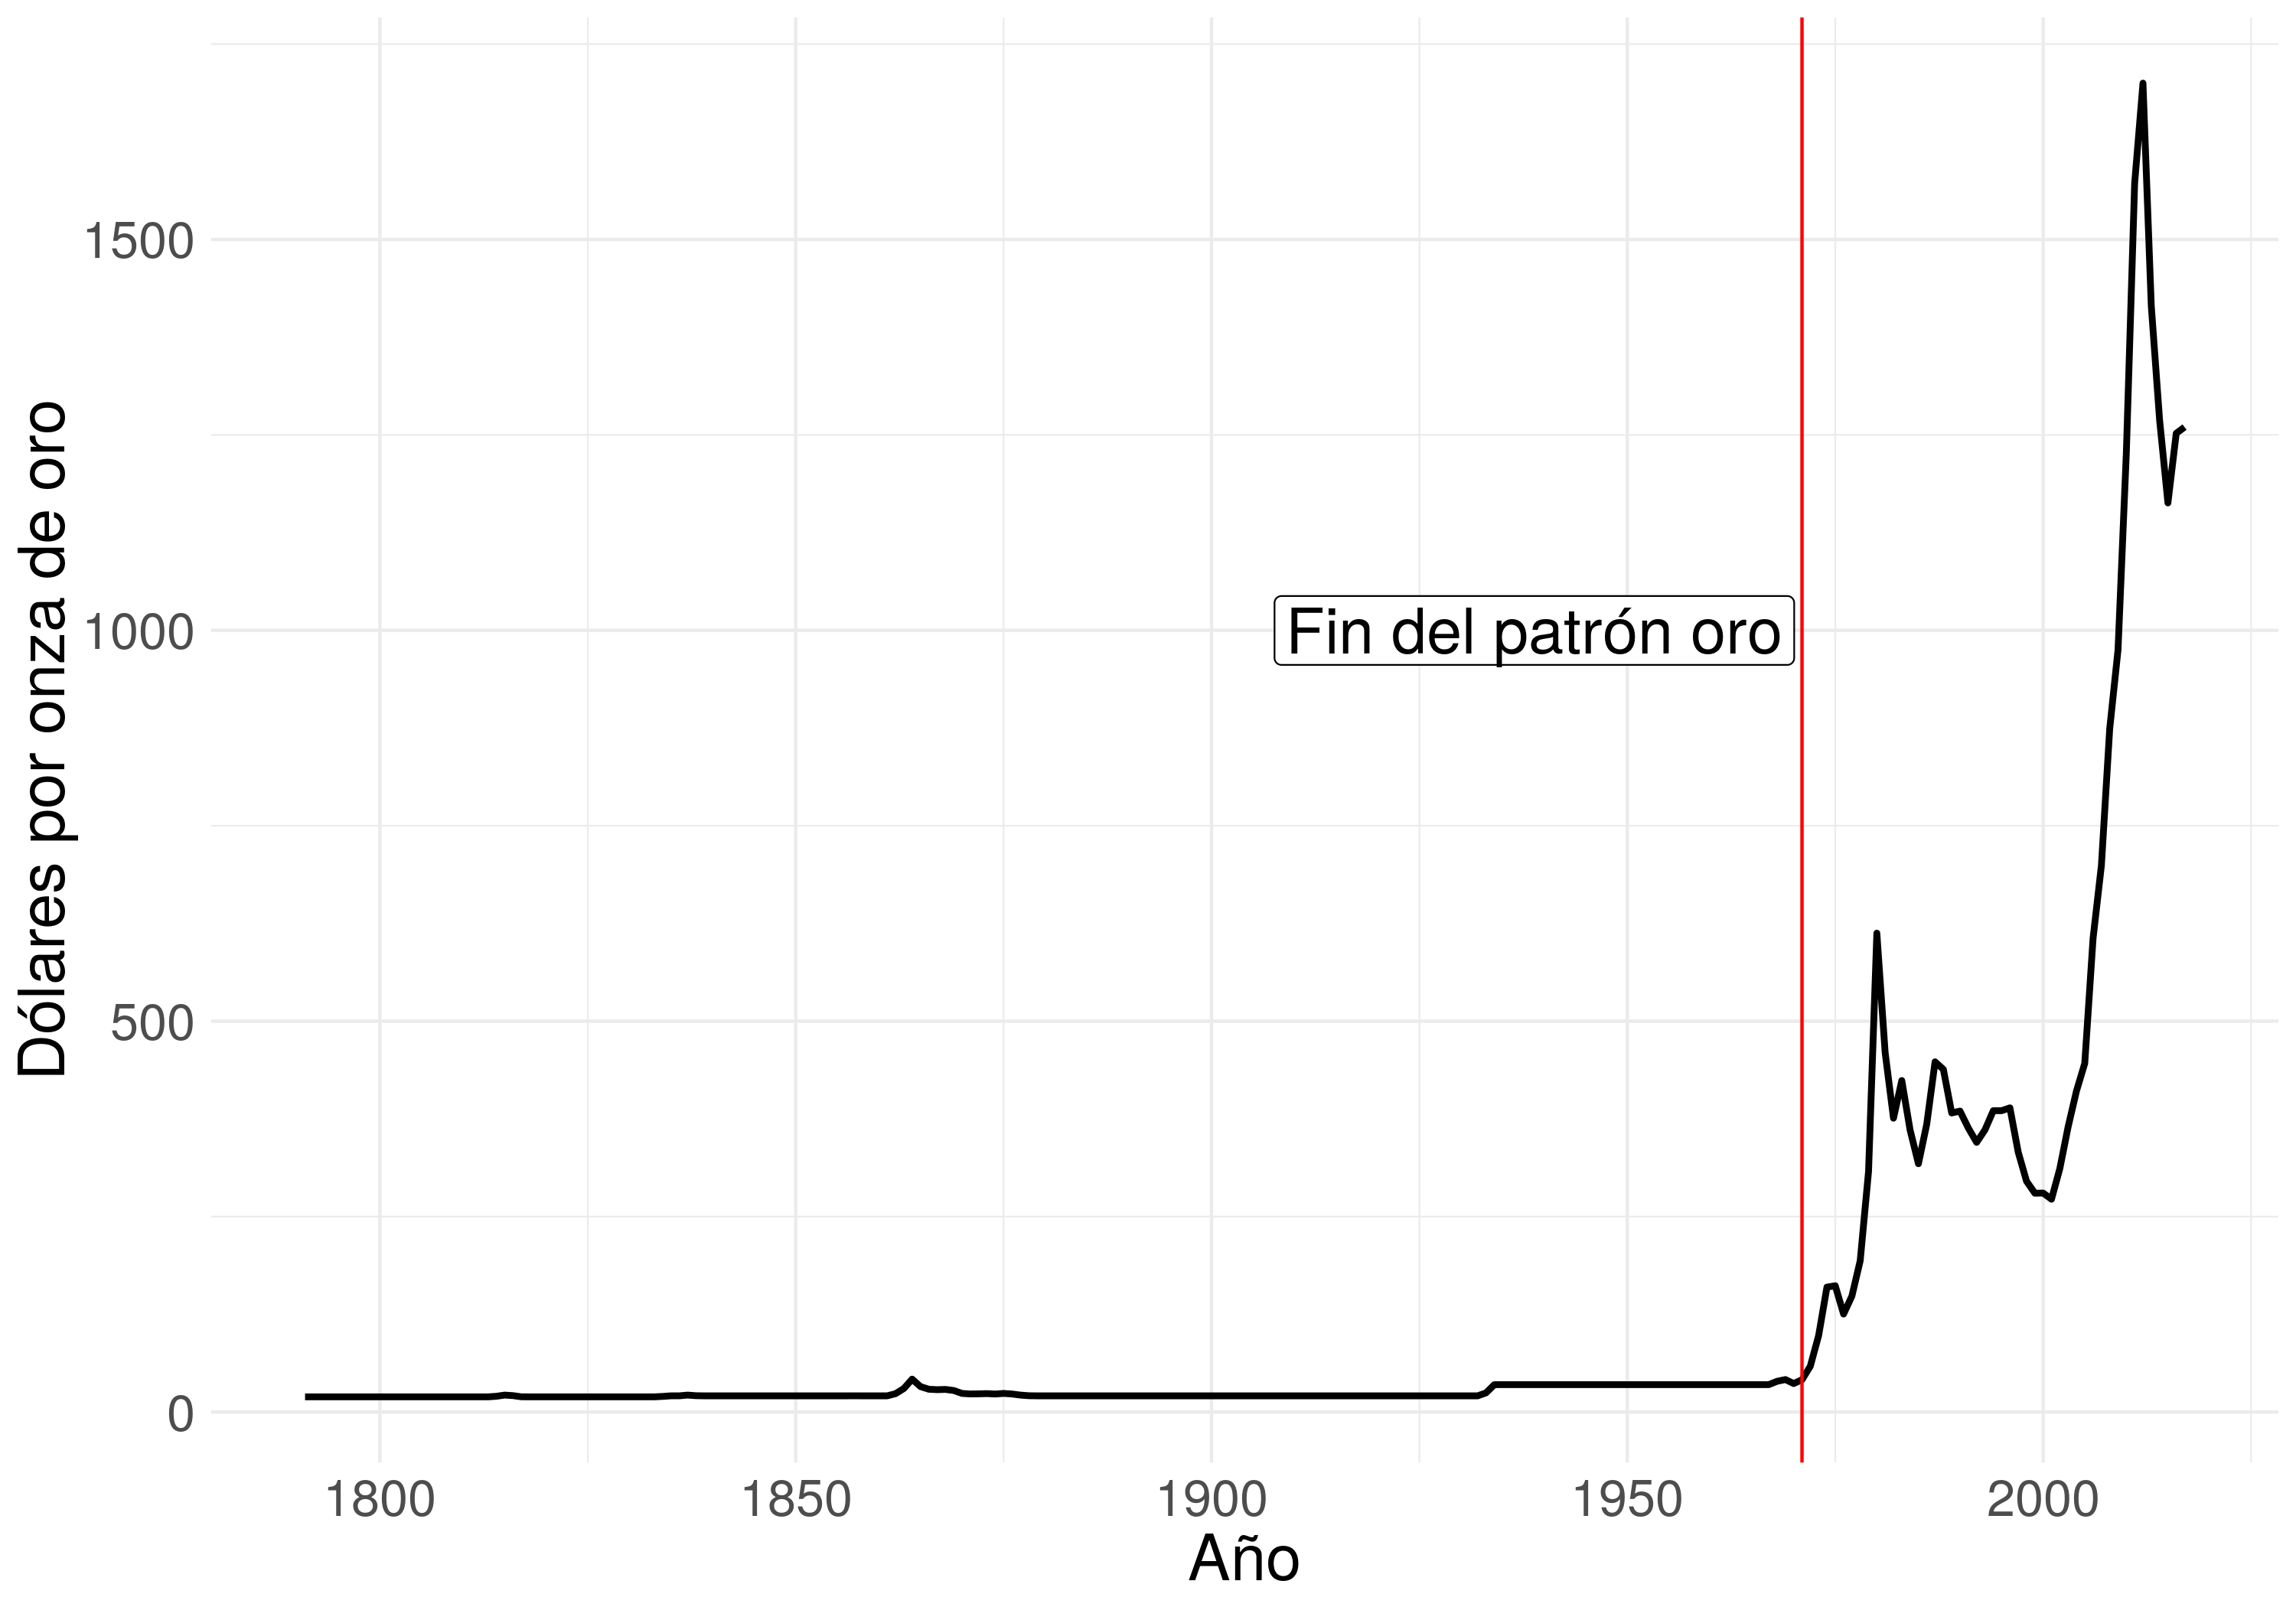
\includegraphics[width=0.75\linewidth]{oro.png}
	 \caption{}\label{fig:oro}
\end{figure}

Dado que lo que se busca en el presente trabajo es realizar un análisis de largo plazo del ciclo económico, esta perturbación nominal oscurece el fenómeno subyacente que se esta intentando captar. Es por ello que se opto por normalizar las series del PBI nominal y el salario nominal por el precio del oro. De esta forma las series se leen como el producto y el salario expresado en su capacidad de compra de oro.
Dado que el oro constituye un refugio de valor en las crisis, su precio es contracíclico, a diferencia de lo que sucede con el Indice de Precios al Consumidor (IPC). De esta manera, al normalizar por el oro en lugar del IPC, se logra una mejor visualización del mismo en las series estudiadas y se facilita el análisis empírico.

% Una alternativa a esto sería dividir por el Indice de Precios al Consumidor, de forma tal que ambas series se expresen en capacidad de poder adquisitivo constante (en términos reales). 
%
%La decisión de expresar el PBI y el salario en capacidad constante de compra de oro y no de poder adquisitivo constante se fundamenta en qué, en tanto el desarrollo de la productividad implica un abaratamiento de la generalidad de las mercancías que componen un indice de precios, y el aumento de la productividad es un fenómeno tendencial de la economía, el PBI expresado en una capacidad de compra constante conserva de forma subyacente una tendencia creciente que oscurece el comportamiento cíclico. El oro, sin embargo, también expresa potencialmente una tendencia al aumento de la productividad en su extracción, no obstante lo cual su precio se encuentra fundamentalmente determinado por el ciclo económico, en tanto constituye un refugio de valor. Este comportamiento contracíclico del precio del oro lo que logra es visibilizar el ciclo en lugar de ocultarlo detrás de una tendencia al aumento de la productividad,y por lo tanto facilita el análisis empírico para el objetivo trazado por el presente trabajo. 

De acuerdo con lo anterior, la figura \ref{fig:PBI} muestra la serie del PBI de Estados Unidos entre el 1900 y 2017, expresado en oro. Por su parte la figura \ref{fig:salario} muestra la serie del salario horario de un obrero de la producción en Estados Unidos entre 1900 y 2017, expresado en oro.

 En ambos casos se resaltan en rojo los períodos de crisis conocidos en la literatura económica, y en líneas punteadas aquellas crisis puntuales que se produjeron en un año particular. La tabla \ref{tabla_crisis} marca el detalle de estas.

\begin{figure}[H]
	\centering
	\subfigure[]{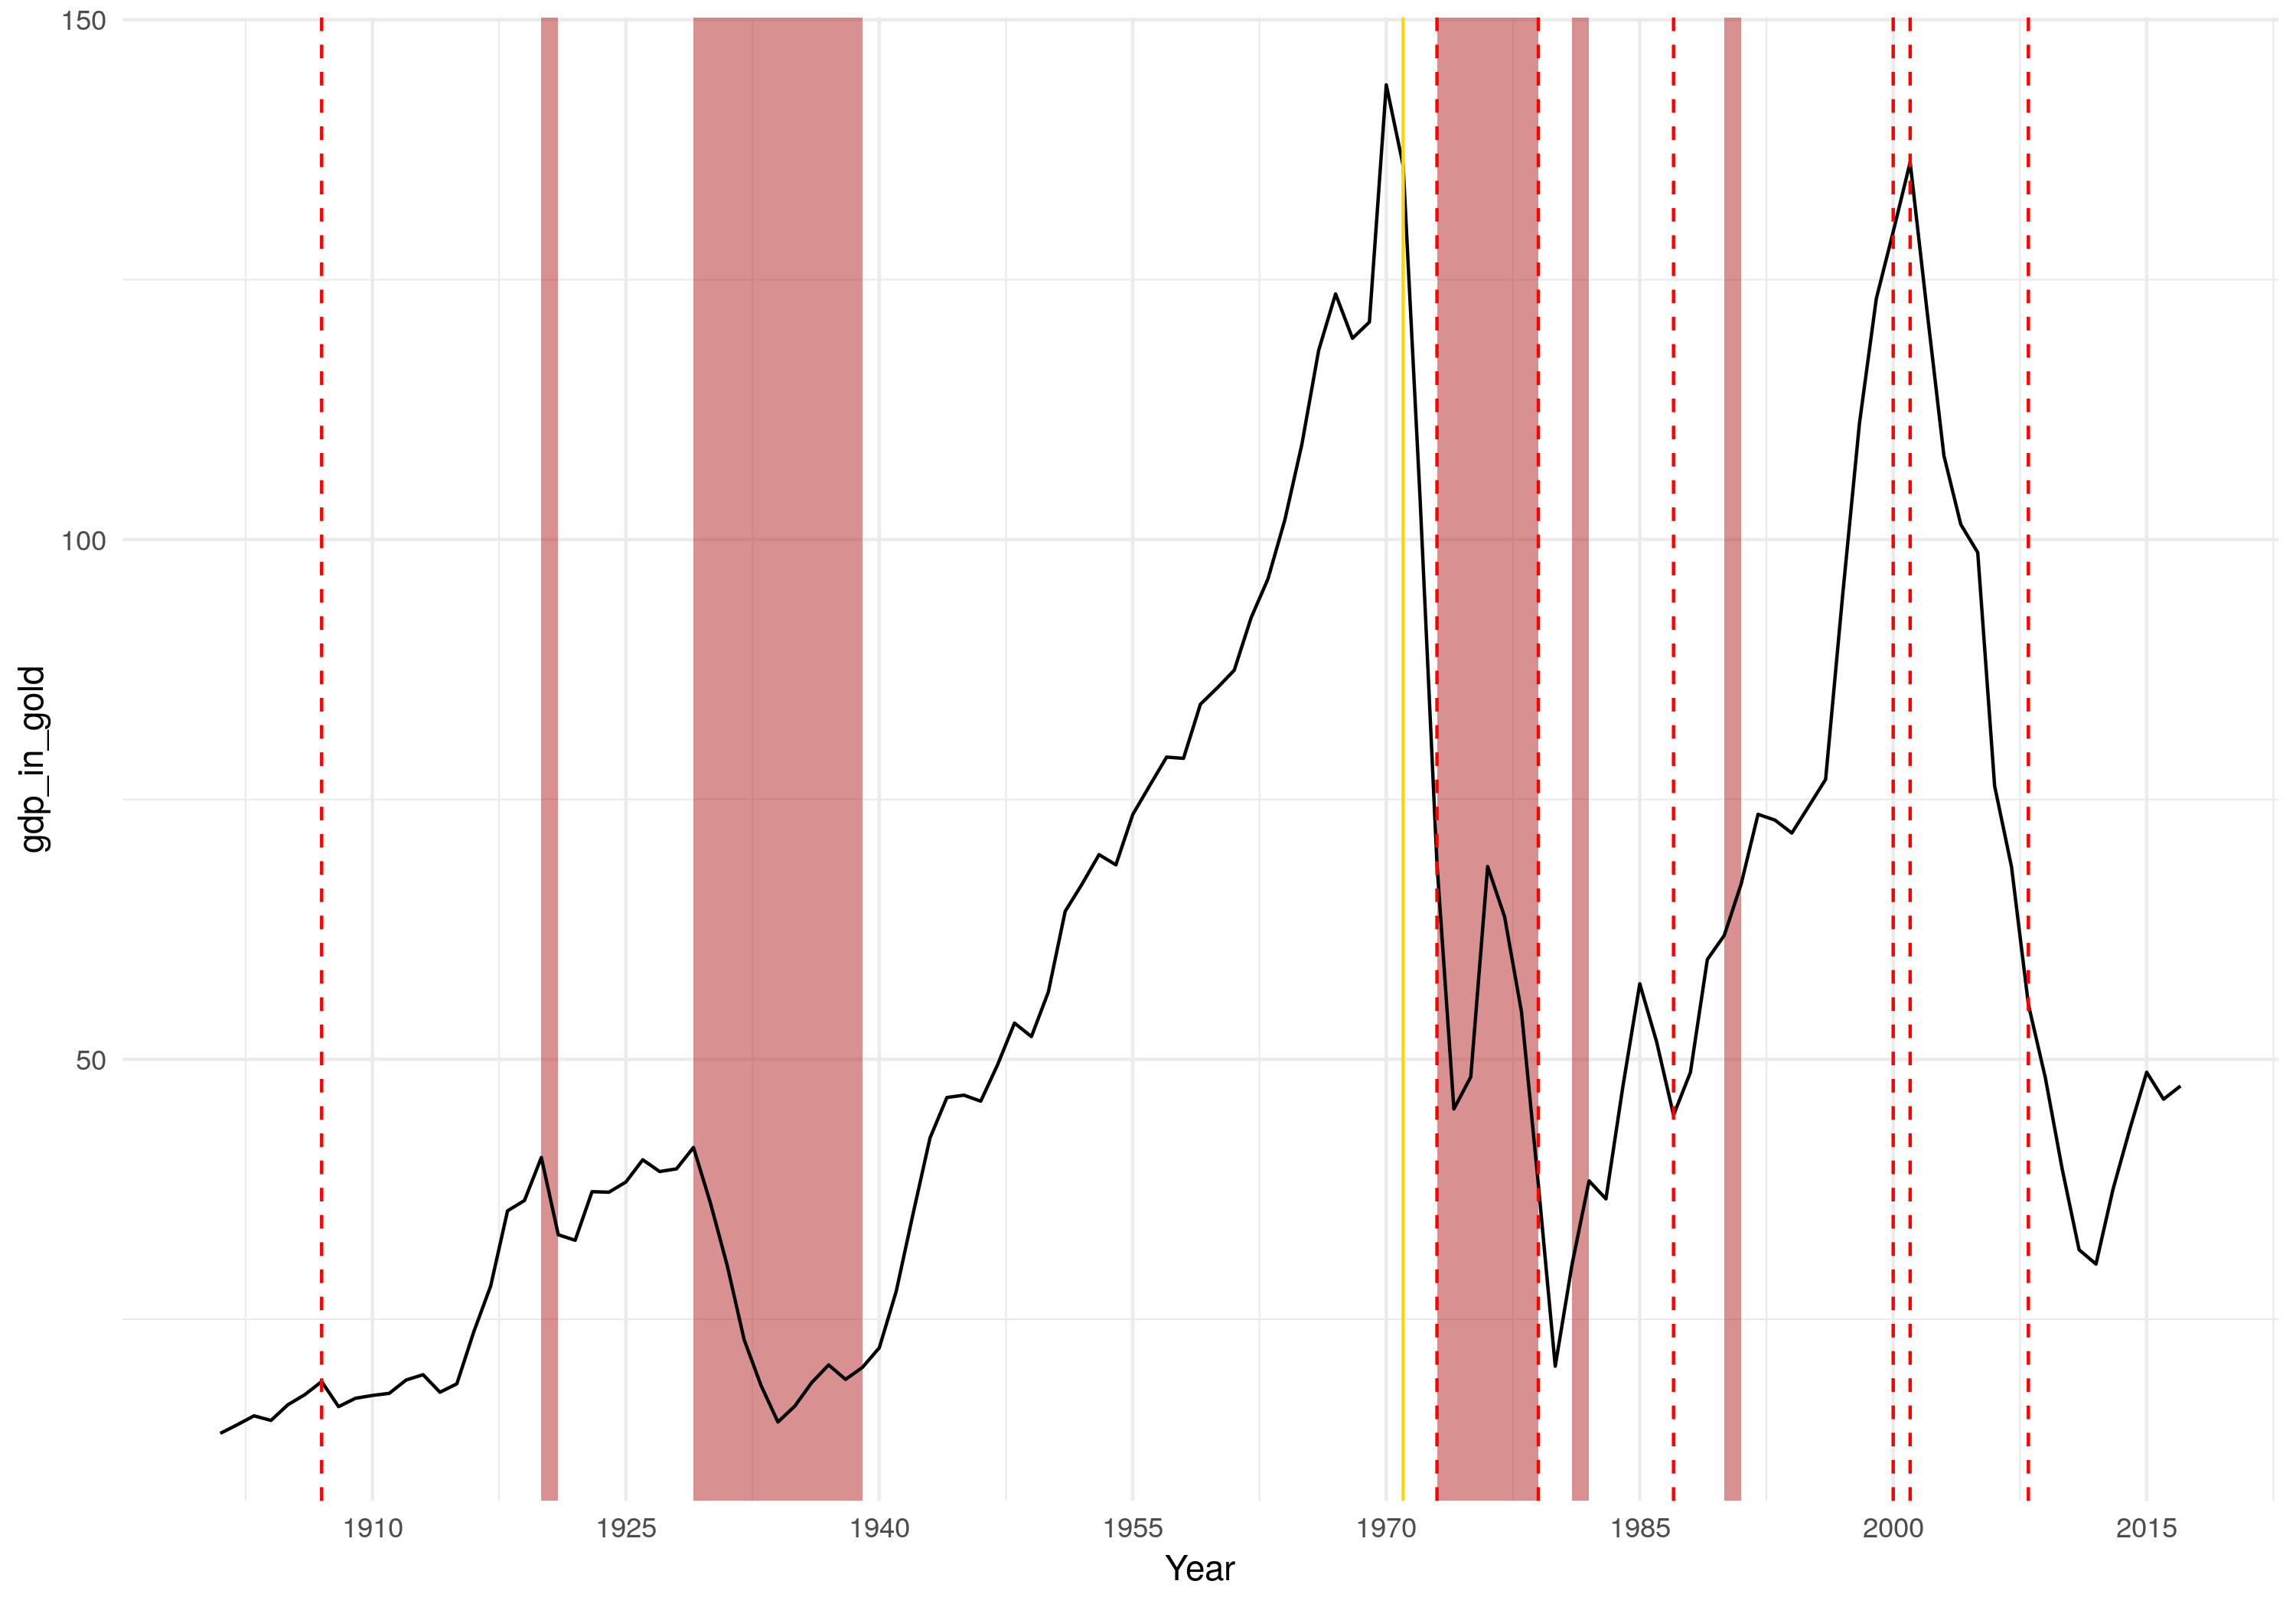
\includegraphics[width=0.75\linewidth]{gdp_in_gold_eda.PNG}
	\label{fig:PBI}}
	\subfigure[]{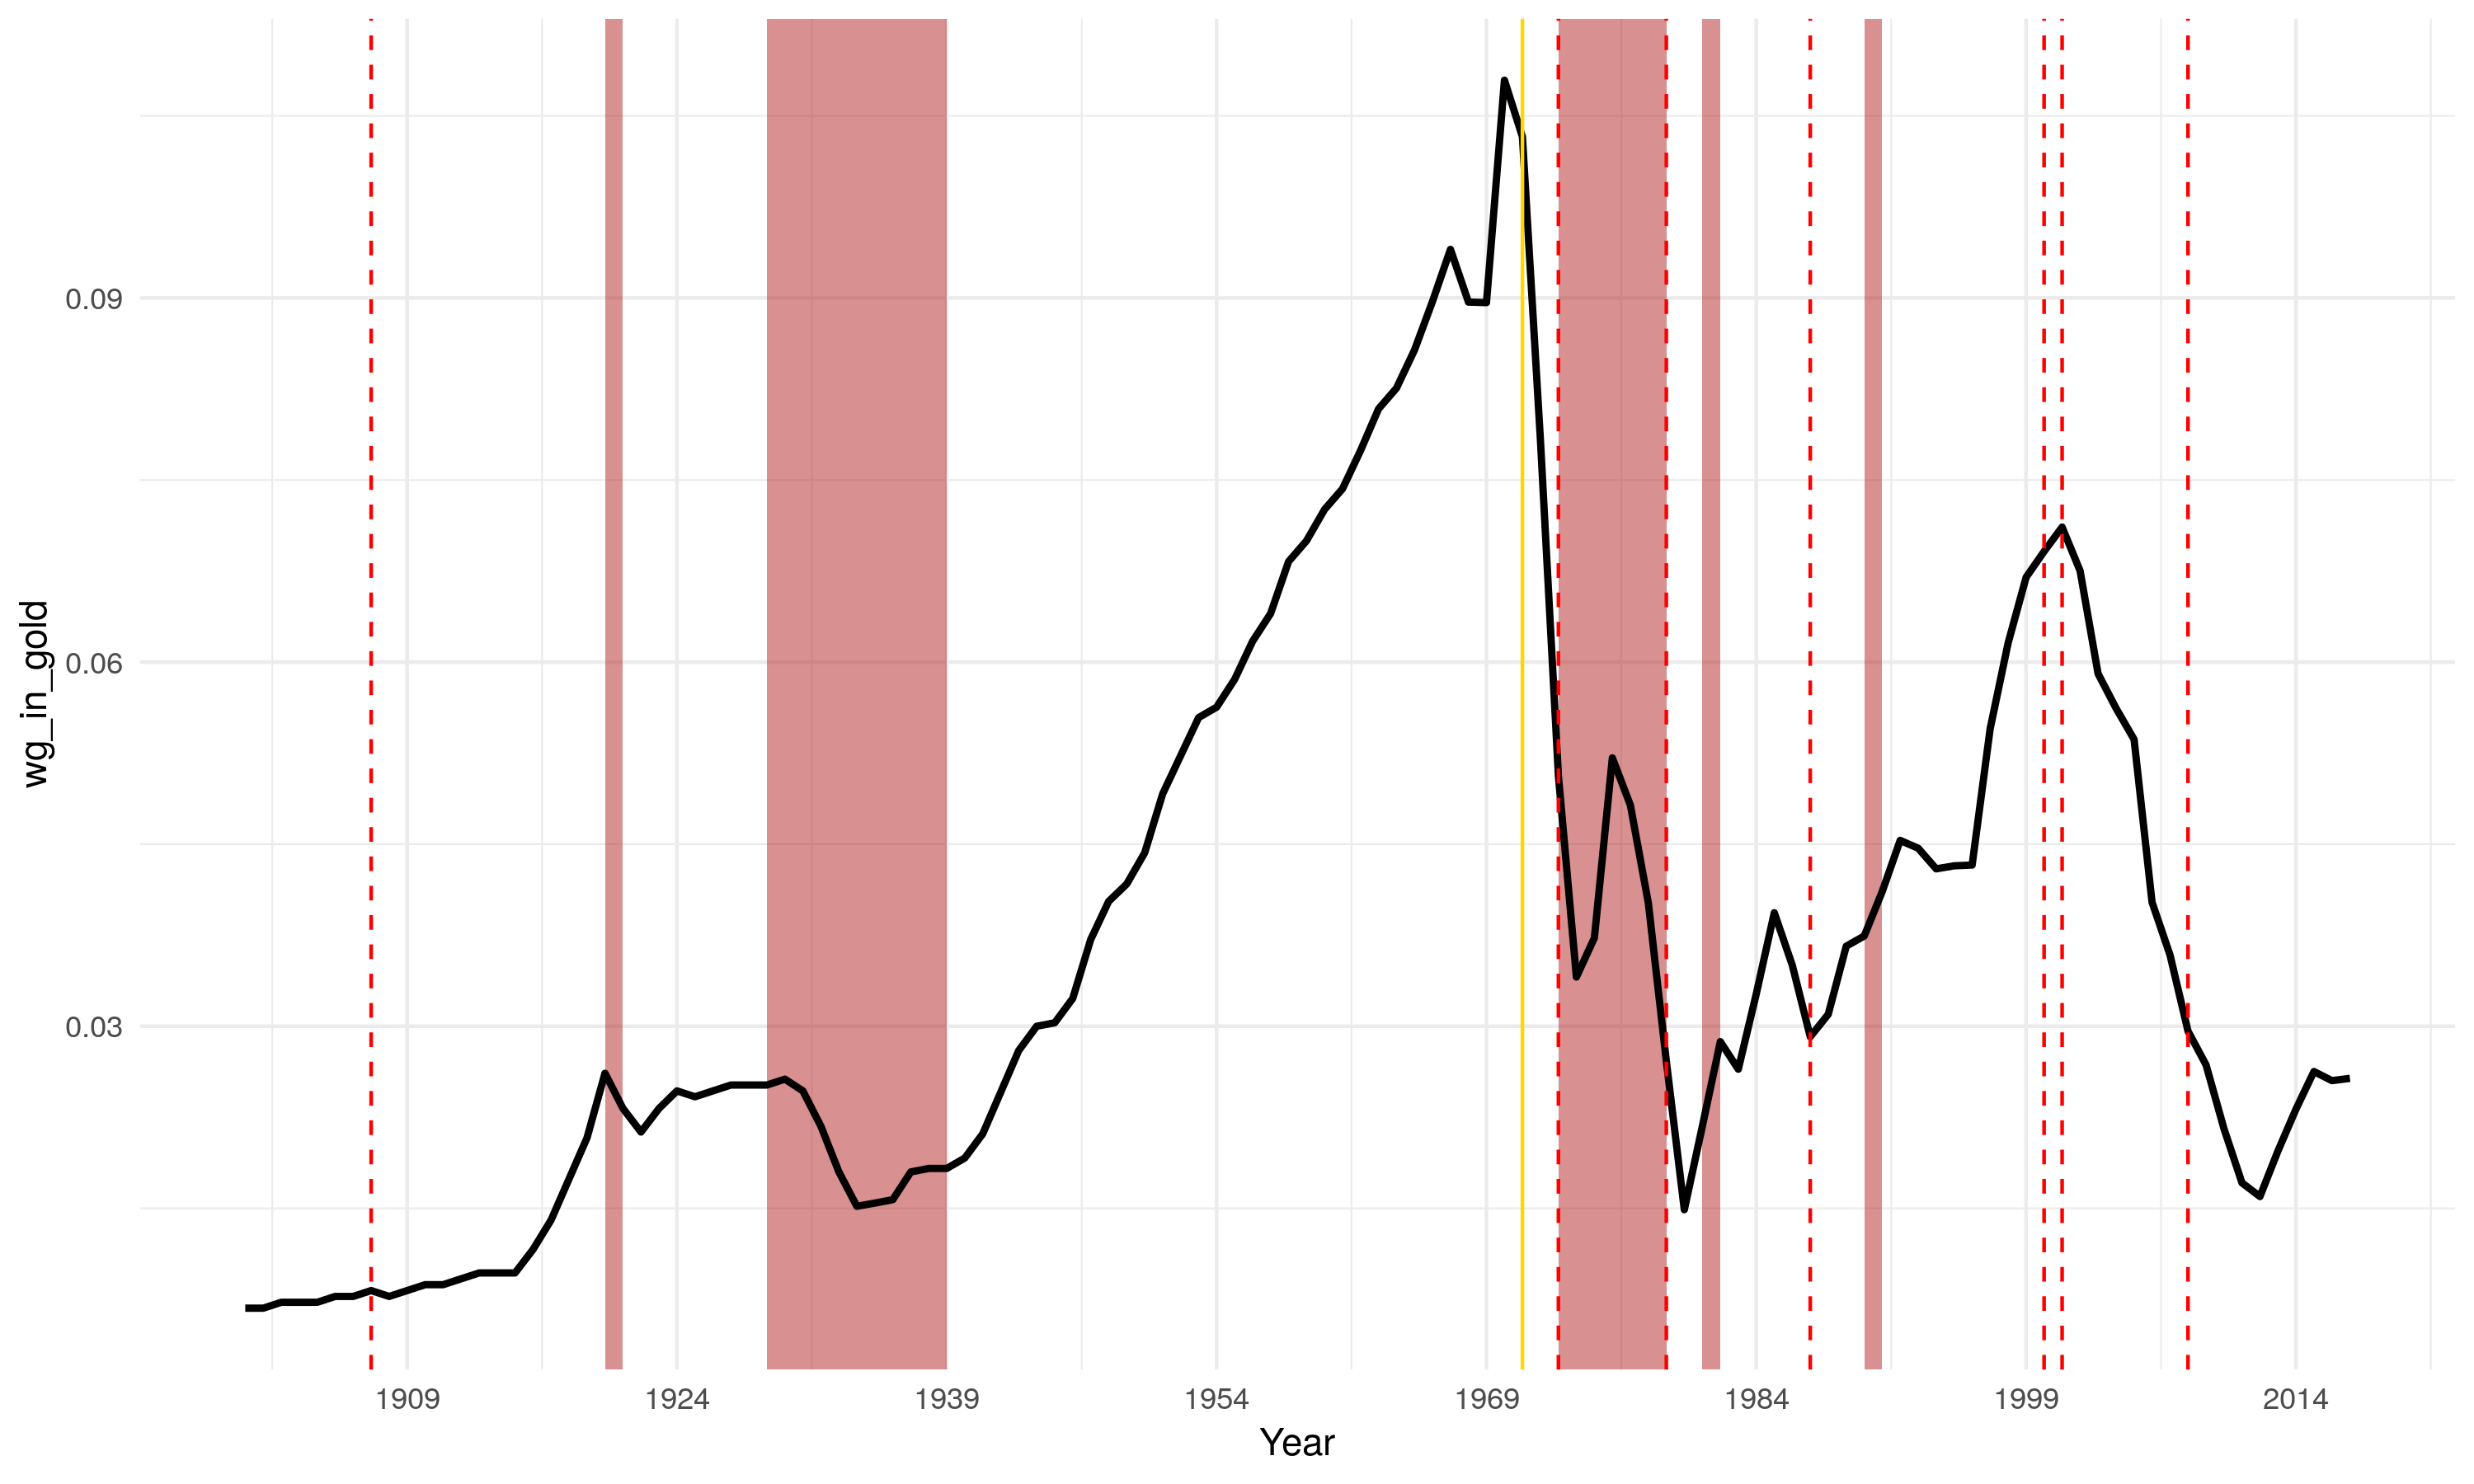
\includegraphics[width=0.75\linewidth]{wg_in_gold_eda.PNG}
	\label{fig:salario}}
	\caption{Series Expresadas en Oro. Destacado de crisis conocidas} \label{fig:series_crisis}
\end{figure}

% latex table generated in R 3.5.1 by xtable 1.8-3 package
% Tue Oct 16 20:07:52 2018
\begin{table}[ht]
	\centering
	\begin{tabular}{ll}
		\hline
		Periodo & Crisis \\ 
		\hline
		1907 & Pánico de 1907 \\ 
		1920 – 1921 & Depresión de 1920 – 21 \\ 
		1929 – 1939 & La gran depresión \\ 
		1970s & 1970s Crisis Energética \\ 
		1973 & Shock de preciso del petróleo de la OPEC(1973) \\ 
		1979 & Revolución Iraní\\ 
		1980s & Recesión de principio de los 80'\\ 
		1987 & Black Monday \\ 
		1990s & Recesión de principio de los 90'\\ 
		2000 & Burbuja de las Dot-com \\ 
		2001 & 911 \\ 
		2008 & Crisis de las subprime \\ 
		\hline
	\end{tabular}
\caption{Principales crisis en EEUU y el mundo.}
\label{tabla_crisis}
\end{table}

En primer lugar lo que se observa es la similitud de ambas series, en términos generales. Ambas muestran tres picos, durante los 20', en 1970 y el 2000, seguidos de caídas profundas. La normalización por el precio del oro permite ver un gran ciclo con tres oscilaciones, por lo menos de manera aparente, durante el siglo XX. Las crisis revisadas por la literatura de historia económica parecen tener su correlato en los movimientos observados en ambas series. Por su parte, también es interesante resaltar que el tercer movimiento ascendente, cuyo punto álgido se encuentra en el año 2000, lleva a un valor similar al del movimiento oscilatorio previo para el caso del PBI, pero no para el salario. Esto expresa que la distribución del PBI en salario y ganancia se modificó en el último período. 

Para complementar el análisis de la serie de Estados Unidos, resulta interesante observar el movimiento del producto en Reino Unido para los centenios precedentes. Durante los siglos XVIII y XIX este país se parapetó como el eje de la acumulación mundial, y por ello resulta de interés buscar evidencias del ciclo económico en este país en particular. En la figura \ref{fig:uk_gdp} se observa el PBI del Reino Unido, entre 1700 y  1900. El mismo se encuentra normalizado por el precio del oro en el mercado londinense para toda la serie a partir de 1718, mientras que los primeros años corresponder al precio oficial británico. A su vez se destacan los años de caída del producto a partir de 1800, dado que para el siglo XVIII no existe visualmente puntos salientes.

\begin{figure}[H]
	\centering
	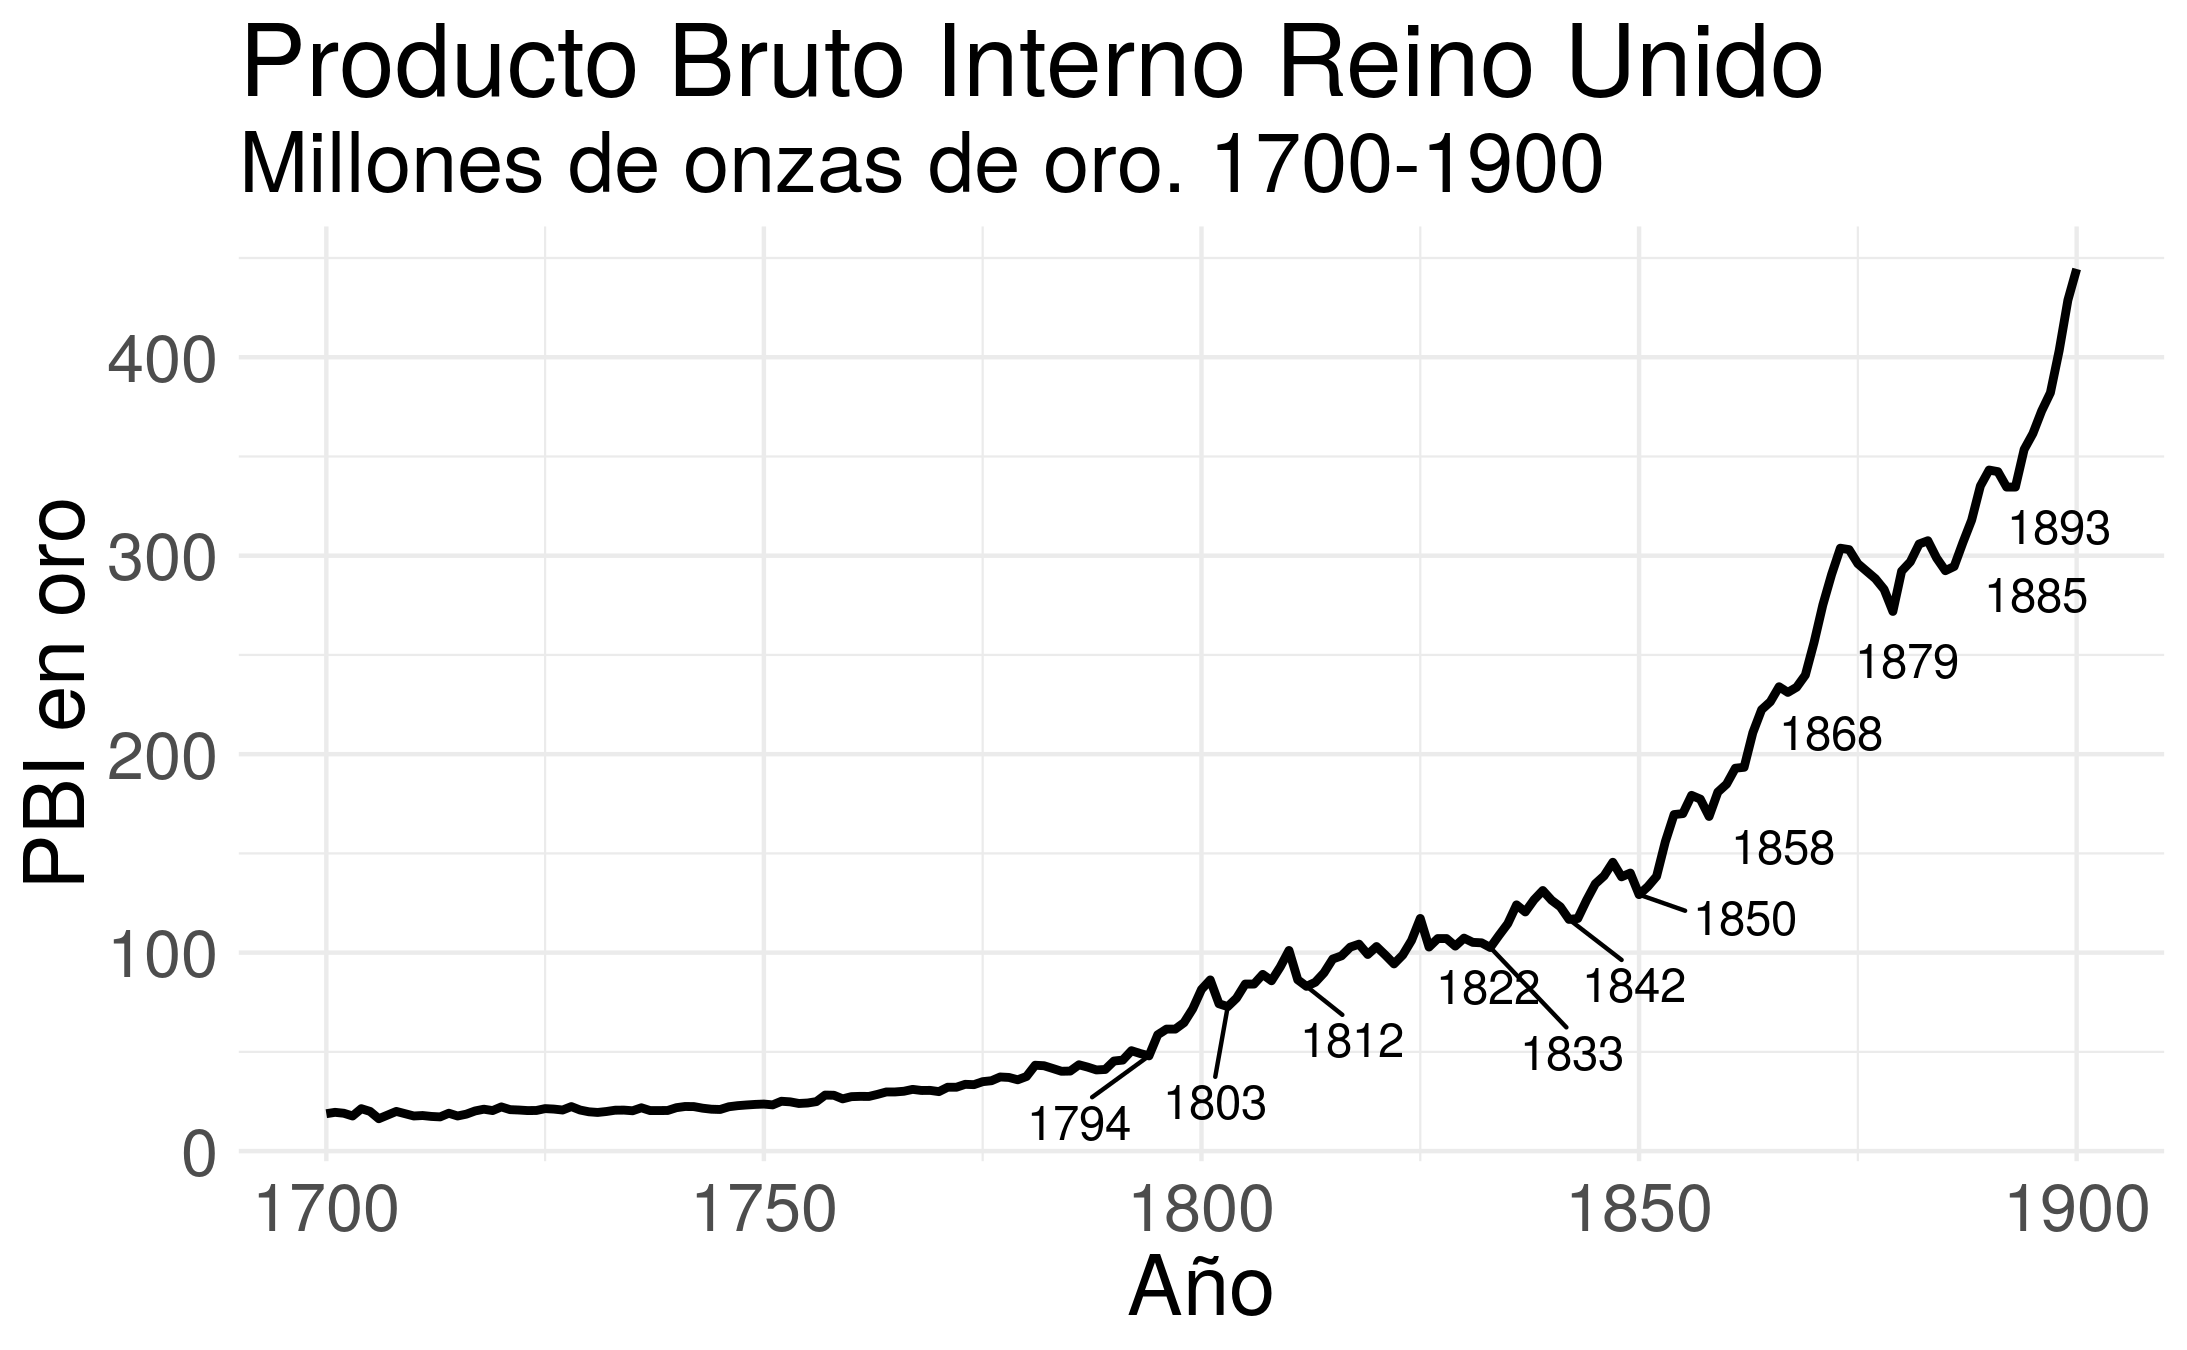
\includegraphics[width=0.75\linewidth]{uk_gdp.png}
	\caption{} \label{fig:uk_gdp}
\end{figure}

Lo que se observa es un movimiento ascendente más suave que el visto para el siglo XX. Vale mencionar que el movimiento del producto en Reino Unido durante el siglo XX conserva una semejanza importante con lo visto para el caso de Estados Unidos. En la figura \ref{fig:uk_gdp} se observa sin embargo un movimiento cíclico en torno a los 10 años de extensión. Durante el siglo XIX se puede notar que cada 7-11 años existe una caída del producto en términos de su capacidad de compra oro. Así como el siglo XX da cuenta de tres grandes oscilaciones, el siglo XIX marca con claridad las oscilaciones más cortas, en torno a los 10 años, mientras que el siglo XVIII en términos relativos expresa una mayor estabilidad. 


En la siguiente sección se utilizaran las series descriptas como insumos para una técnica proveniente del campo de procesamientos de señales, los Wavelets, que permite destacar de forma automática las amplitudes cíclicas más importantes de la serie.

\section{Wavelets}

Si bien en la econometría es extendido el uso de modelos autoregresivos y de medias móviles para el análisis de series de tiempo, existe en la literatura de análisis de señales otras técnicas de amplia difusión que aún no son de uso generalizado en el estudio de series económicas. Un ejemplo clásico en este sentido son las series de Fourier. En este campo de estudio se analiza como cualquier serie de tiempo se puede pensar como una composición de funciones periódicas, es decir como la suma de senos y cosenos. De esta forma, se construye un espacio de \textit{frecuencia} ($1/periodo$) donde se definen las funciones periódicas en función de su frecuencia (o extensión en el tiempo, movimiento horizontal) y amplitud (movimiento vertical). En la figura \ref{fig:ciclo} se puede observar estas definiciones.

\begin{figure}[H]
	\centering
	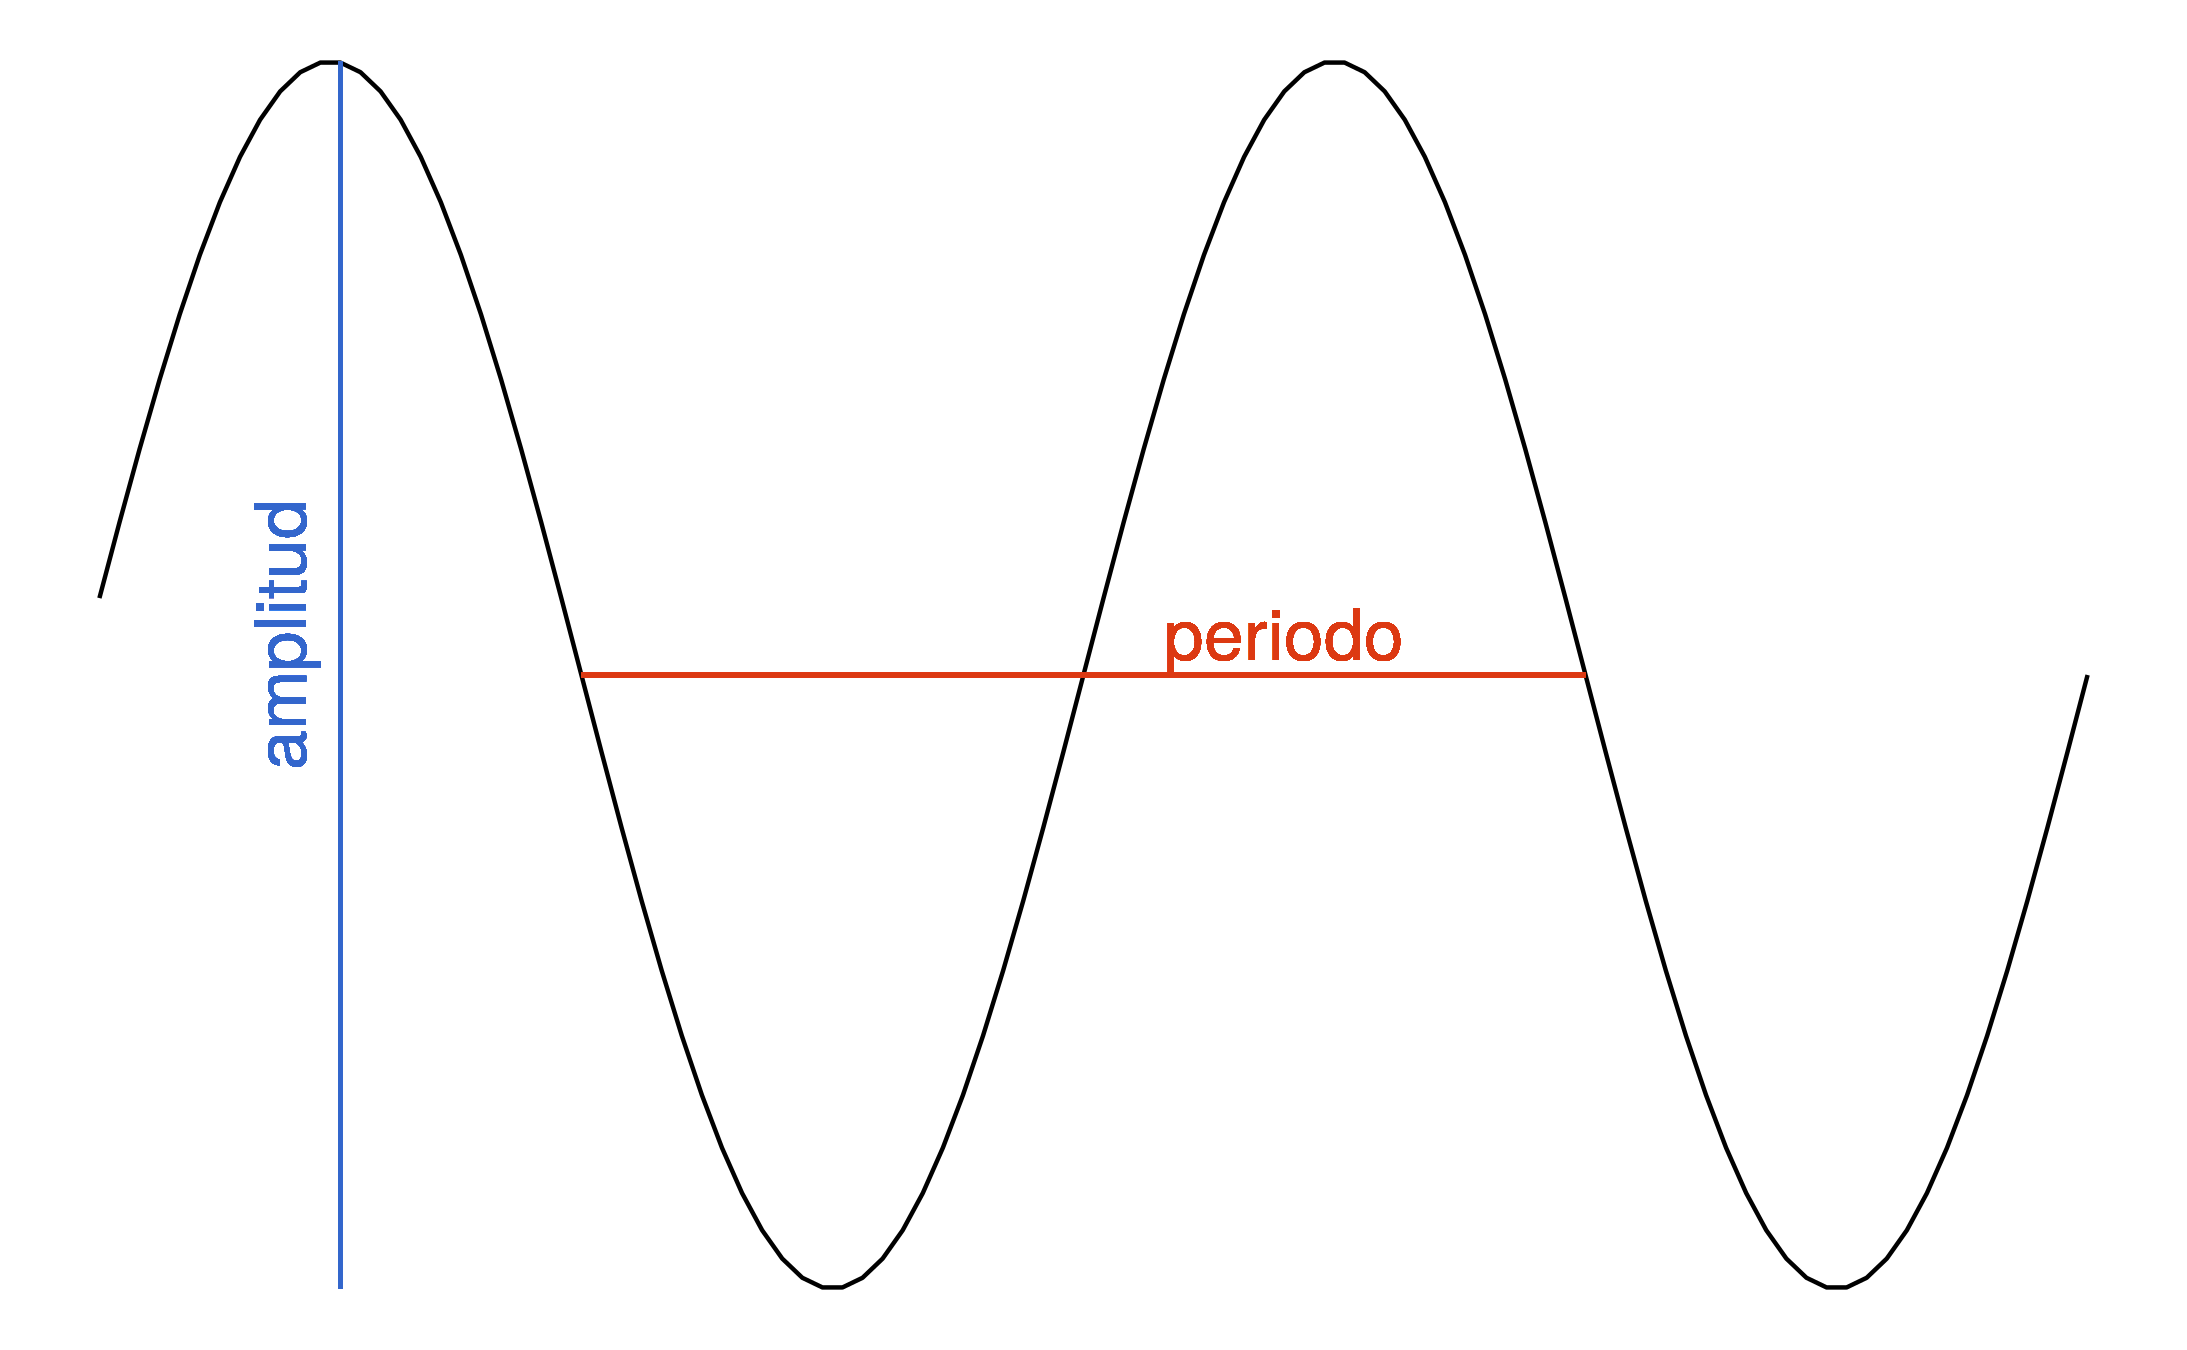
\includegraphics[width=0.65\linewidth]{ciclo.png}
	\caption{período y amplitud} \label{fig:ciclo}
\end{figure}

La descomposición de Fourier se basa en una transformación del dominio de la serie, desde el dominio del tiempo, al dominio de la frecuencia.\\

Las wavelets también son un tipo de transformación sobre la serie original que puede pensarse como una rotación de un espacio de funciones a un dominio diferente. Pero a diferencia de la transformada de fourier que tiene como base de funciones los senos y cosenos, la transformada Wavelet tiene como base de funciones una tipo particular, denominadas Wavelets \cite{castro1995wavelets}. Una base de este tipo se construye a partir de una función madre, que es una onda corta, de duración finita. Es decir, a diferencia de las funciones seno y coseno que se extienden infinitamente, los wavelets tienen \textit{soporte compacto}, es decir que utilizan como base funciones que no se extienden infinitamente en el dominio del tiempo. Otra característica de las funciones wavelet es que el área debajo de la curva debe ser igual a cero, es decir que esta centrada en cero. Esta función madre se traslada y dilata para construir una base ortonormal. 

Mientras que una transformación de Fourier de una serie desde el dominio del tiempo hacia el dominio de la \textit{frecuencia} toma la forma de:

$$
X(F)=\int_{-\infty}^{\infty} x(t) e^{-j2\pi Ft}dt
$$

La transformada wavelet lleva del dominio del tiempo al dominio de \textit{escala} y \textit{traslación}:

$$
X(a,b)=\int_{-\infty}^{\infty} x(t) \psi^*_{a,b}(t)dt
$$

La escala describe la frecuencia (inversa de la extensión o período) del ciclo, mientras que la traslación describe el movimiento a lo largo de la serie. Dado que las series de baja frecuencia (ciclos más largos) ocupan una porción mayor de la serie, son más difíciles de ubicar en un momento particular del tiempo. Por esto último, la resolución en bajas frecuencias es mala en el dominio del tiempo, pero buena en el dominio de la frecuencia, mientras que los ciclos de alta frecuencia tienen alta resolución en el dominio del tiempo, pero menos resolución en el dominio de la frecuencia.Si lo comparamos con las transformadas de fourier, podríamos pensar que ésta tiene muy alta resolución en el dominio de la frecuencia, pero ninguna resolución en el dominio del tiempo. El wavelet logra definir la presencia de una determinada frecuencia en un determinado momento del tiempo.
 

También es posible entender a los Wavelets como un análisis de la correlación entre una serie de tiempo, y una cierta función ondulatoria compacta, en un momento del tiempo y una frecuencia determinada. Las traslaciones lo que generan es un corrimiento de la función ondulatoria, y por lo tanto podemos calcular la correlación para todo el rango temporal. El reescalado modifica la frecuencia de la función ondulatoria, lo que permite calcular la correlación para varias frecuencias de onda diferentes. La cantidad de datos disponibles es la que define la capacidad de reescalar la función base, es decir, cuan bajas son las frecuencias mínimas que se puede analizar. Finalmente lo que obtenemos es un valor de la asociación lineal entre la serie original y la función base, para cada valor del tiempo y la frecuencia.  

La función base que utilizamos para el presente trabajo es la denominada \textit{Morlet Wavelet}, que tal como se implementa en la librería WaveletComp \citep{Roesch2018} tiene la siguiente forma funcional:
$$
\psi(t)=\pi^{-\frac{1}{4}}e^{i\omega t}e^{\frac{-t^2}{2}}
$$

Donde $\omega$ es la frecuencia angular (tasa de rotación en radianes por unidad de tiempo). Esta es una función continua, compleja, frecuentemente utilizada en la literatura \citep{conraria2011continuous}. Por su parte, las base a partir de la traslación, $a$, y el escalado, $b$, implementada es:

$$
X(a,b)=\sum_{t} x(t)   \frac{1}{b} \psi^*\left(\frac{t-a}{b}\right)dt
$$

Visualmente, las traslaciones y reescalados de la función base se pueden observar en la figura \ref{fig:morlet}. Allí se aprecia que las traslaciones se definen en el dominio del tiempo, mientras que los reescalados lo hacen en el dominio de la frecuencia. Luego, si se reconstruye el plano tiempo-frecuencia y se calcula la correlación de cada punto del dicho plano con la serie original, se obtiene una nueva dimensión que representa el grado de ajuste de nuestra serie a cada frecuencia, para los distintos momentos del tiempo. 

\begin{figure}[H]
	\centering
	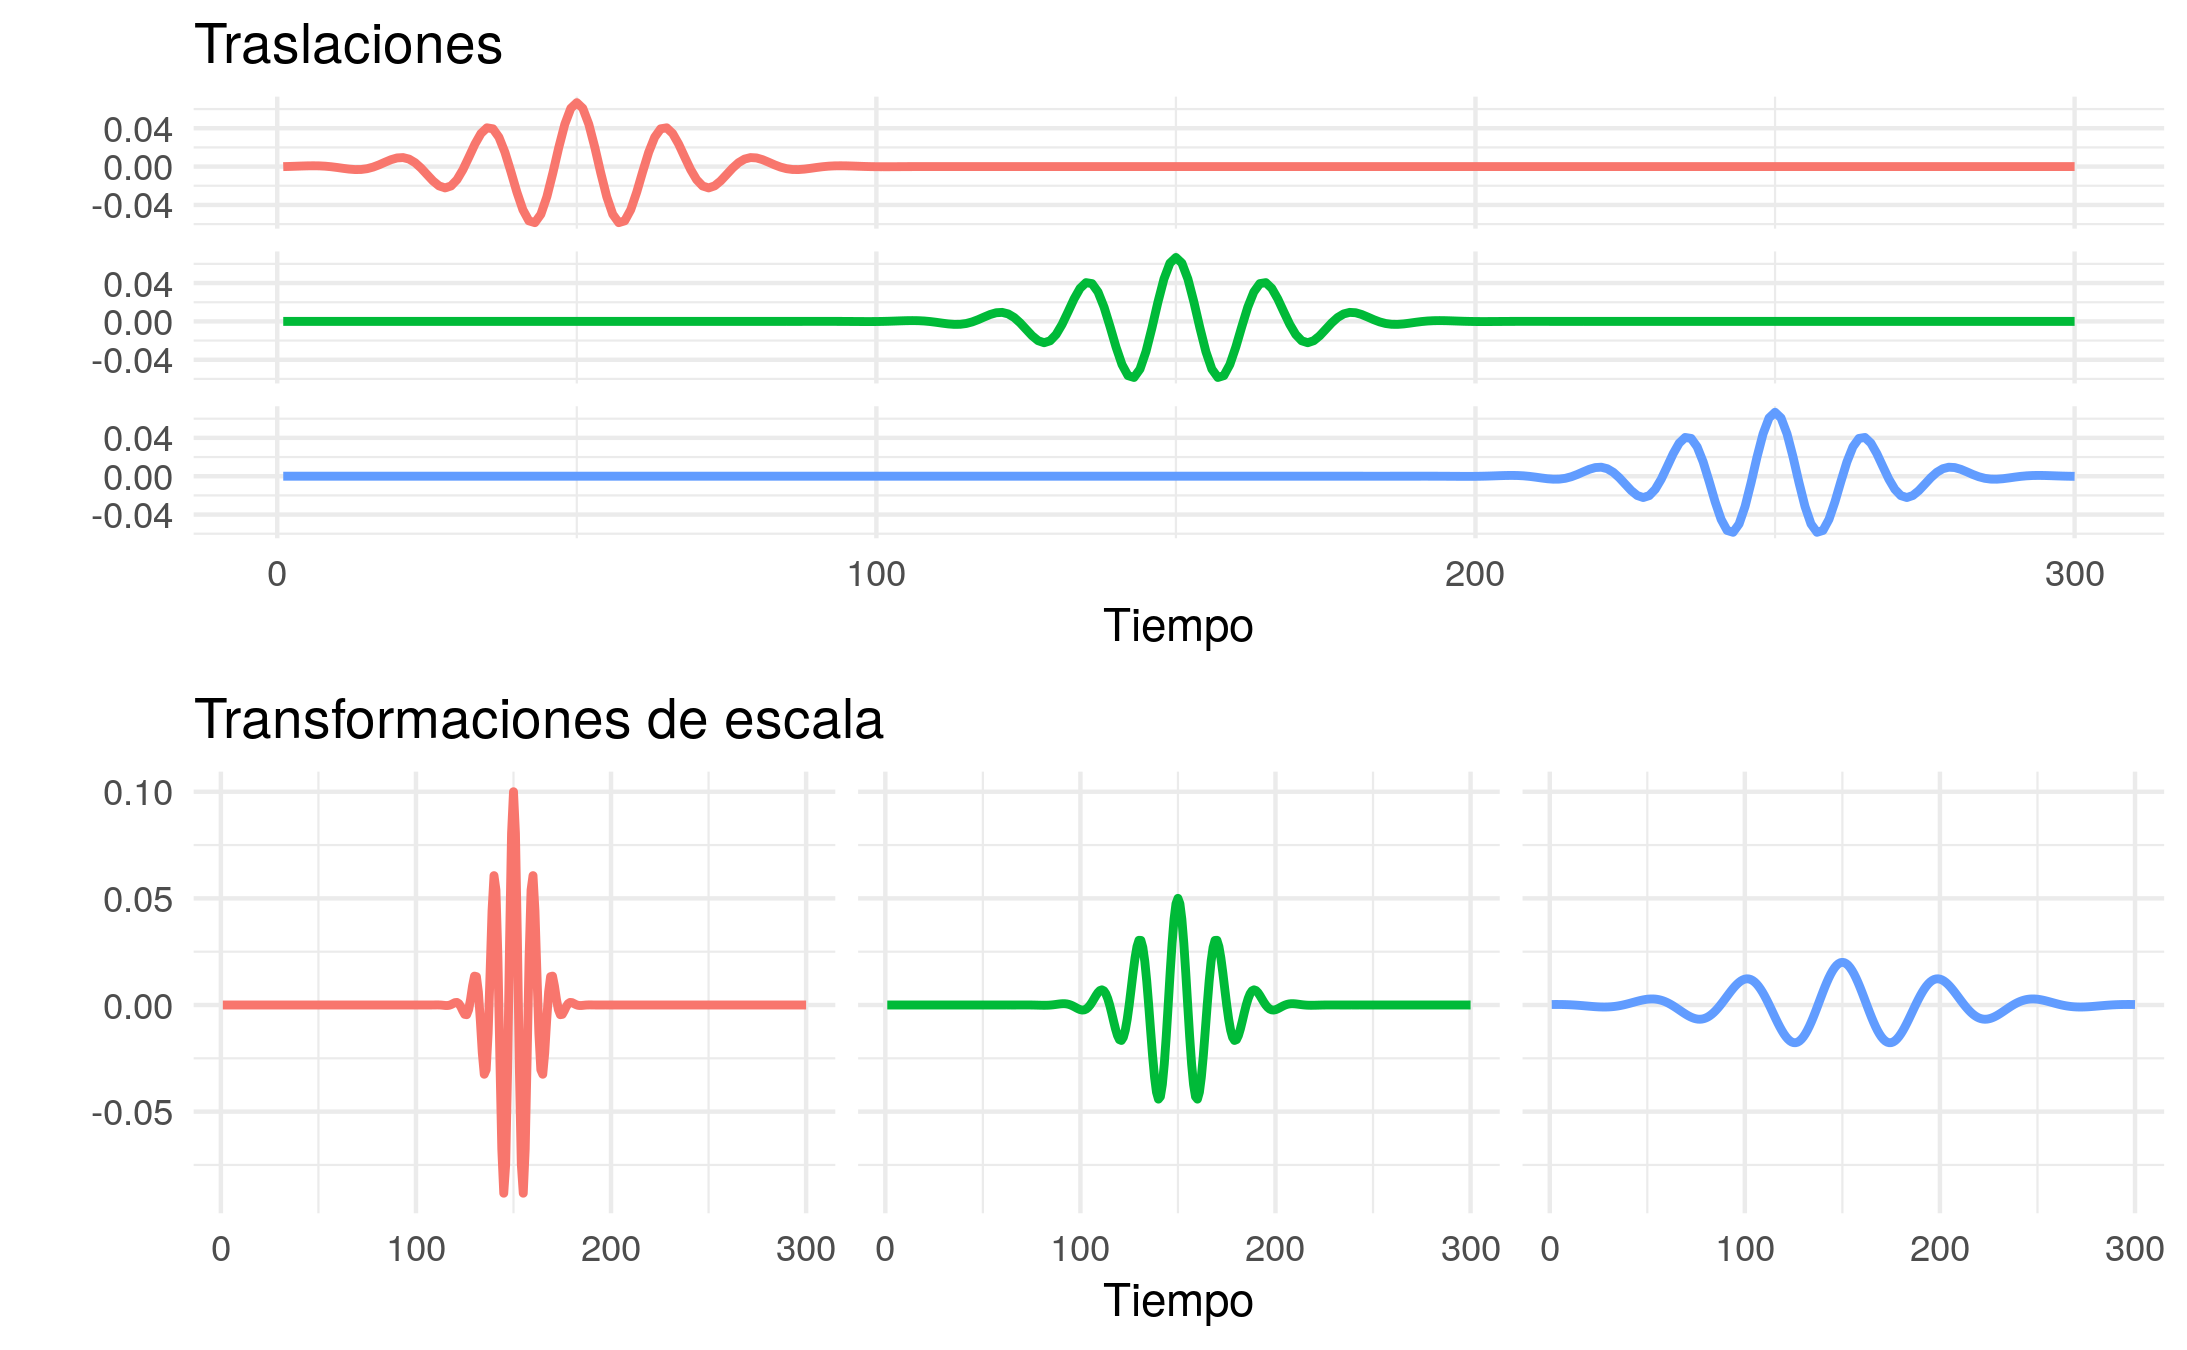
\includegraphics[width=\linewidth]{morelt.png}
	\caption{Traslaciones y reescalados de la función base Morlet} \label{fig:morlet}
\end{figure}


Finalmente, los resultados los podemos visualizar en un \textit{espectograma}, es decir, podemos ver para cada frecuencia, en cada momento del tiempo, el grado de correlación de la serie original con la función morlett en dicho punto.


Para visualizar las wavelets en el análisis del ciclo económico es útil definir un modelo teórico de una economía cíclica, con los diferentes componentes vistos por separado y en su composición, para observar las características del espectograma en este modelo,  y luego compararlo con los datos reales. 
En la figura \ref{fig:serie_teorica} se observan 100 valores de los distintos componentes con los que construiremos la serie, los mismos son:

\begin{itemize}
	\item \textbf{impulso}: Una serie con un valor constante de 50, que en período en particular tomar el valor 100.
	\item \textbf{Tendencia}: Crece medio punto por período.
	\item \textbf{ciclo corto}: Un ciclo de amplitud y extensión pequeña
	\item \textbf{ciclo medio}: Un ciclo de amplitud y extensión media
	\item \textbf{ciclo largo}: Un ciclo de amplitud y extensión grande
	\item \textbf{ruido}: Ruido generado a partir de una distribución normal, poco significativo respecto a la amplitud de los ciclos y la pendiente de la tendencia.
\end{itemize}

En código R, los elementos de la serie teórica se pueden expresar de la siguiente manera:

\begin{lstlisting}
n = 1000
impulso= c(rep(50,(n/2-1)),100,rep(50,n/2))
tendencia = c(1:n)/2
corto = 10 * sin(( 2 * pi/3 ) * c(1:n))
medio = 20 * sin(( 2 * pi/10) * c(1:n))
largo = 30 * sin(( 2 * pi/50) * c(1:n))
ruido <- rnorm(n)
serie_compuesta = impulso + tendencia + corto + medio + largo + ruido
\end{lstlisting}


\begin{figure}[H]
	\centering
	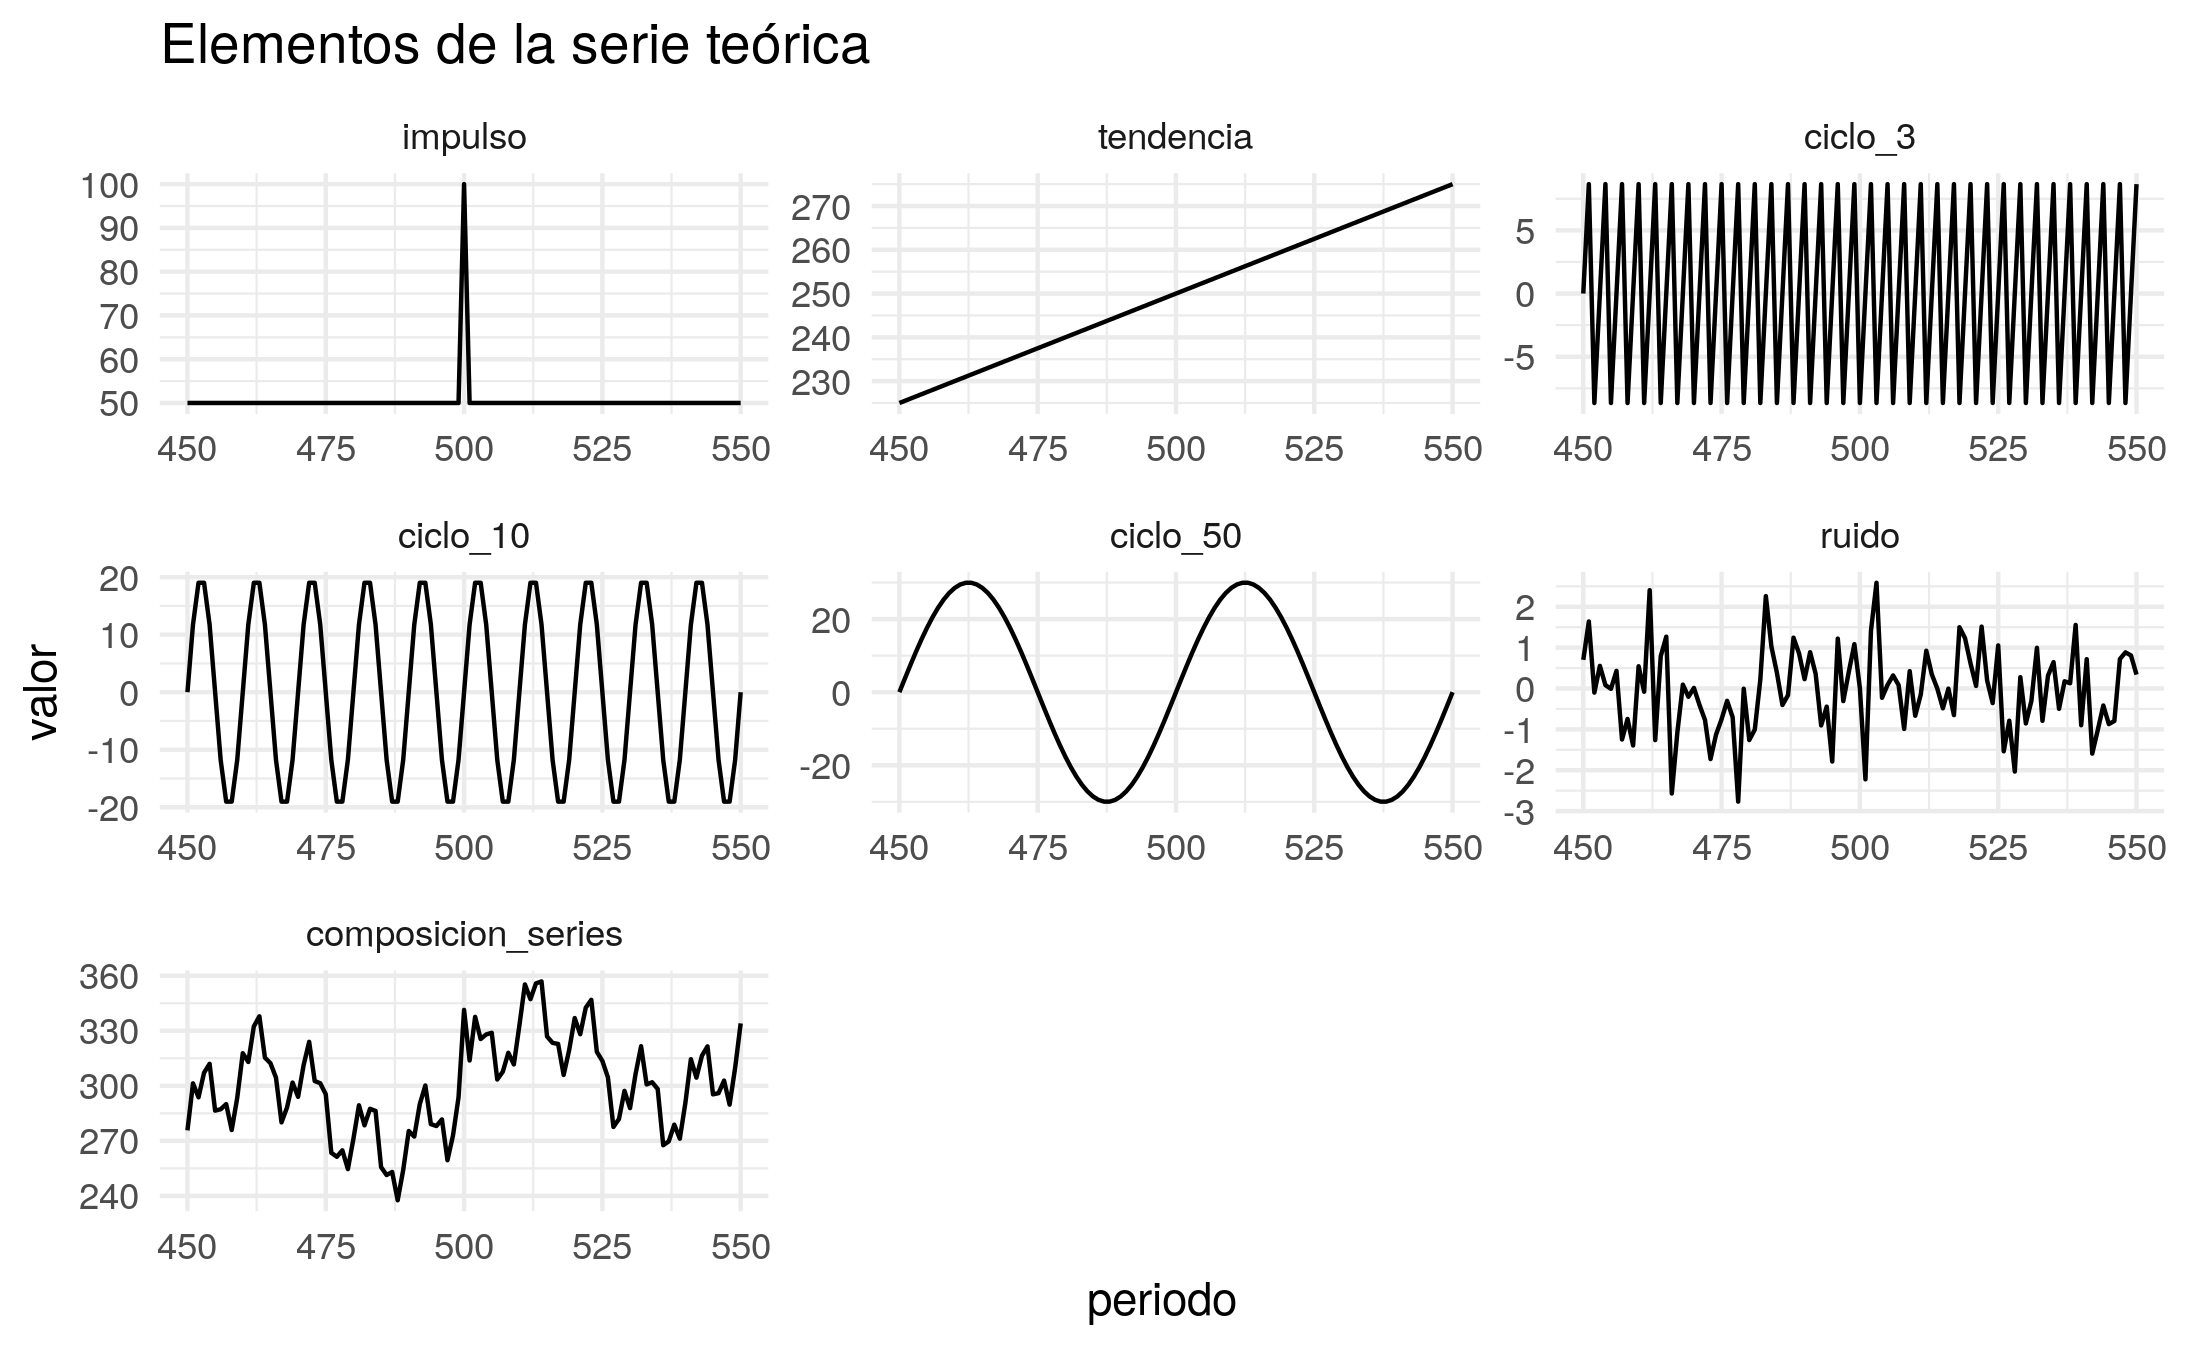
\includegraphics[width=\linewidth]{serie_teorica.PNG}
	\caption{} \label{fig:serie_teorica}
\end{figure}

En la figura \ref{fig:espect_teo} se observa el espectograma de cada uno de los elementos mencionados. Dicho gráfico muestra en el eje vertical el período, la inversa de la frecuencia de onda, que corresponde a la distancia entre los valles o picos de un ciclo. La escala cromática (de los azules para los valores más bajos a los rojos en los valores más altos) representa la amplitud del ciclo. el eje horizontal representa el tiempo calendario. Es decir, para cada tiempo calendario podemos observar la amplitud del ciclo en cada una de las posibles frecuencias de onda. 

\begin{figure}[H]
	\centering
	\subfigure[impulso]{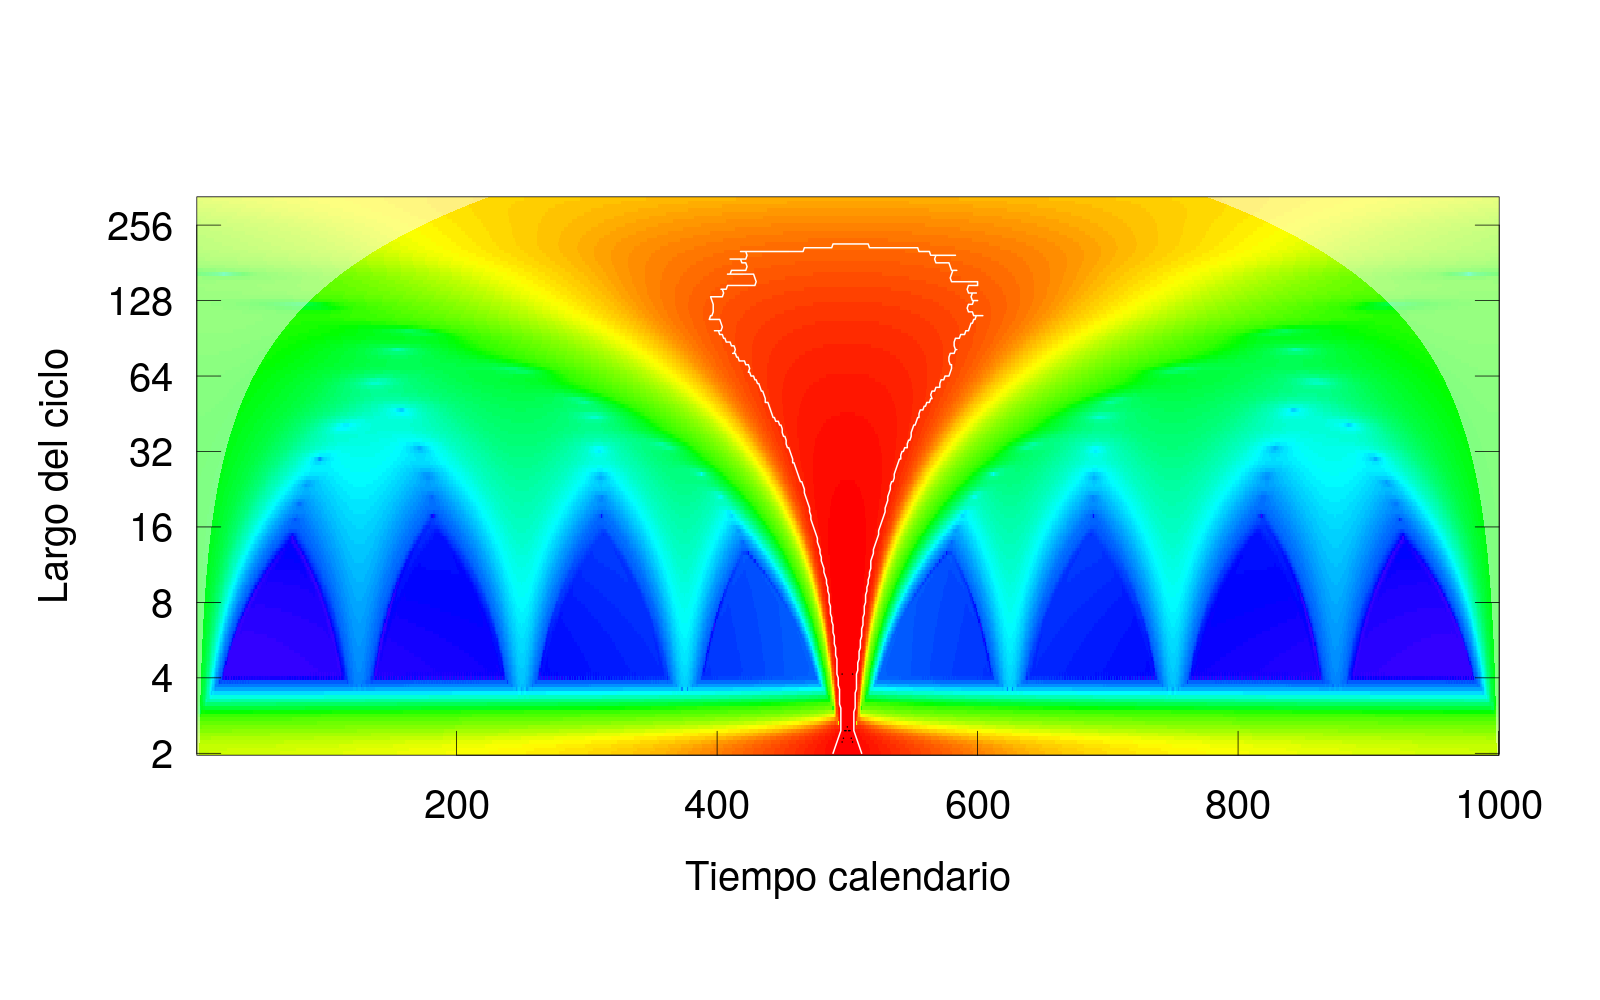
\includegraphics[width=0.49\linewidth]{espectograma_teorico_impulso.png}}
	    \vspace{0.00mm}
	\subfigure[tendencia]{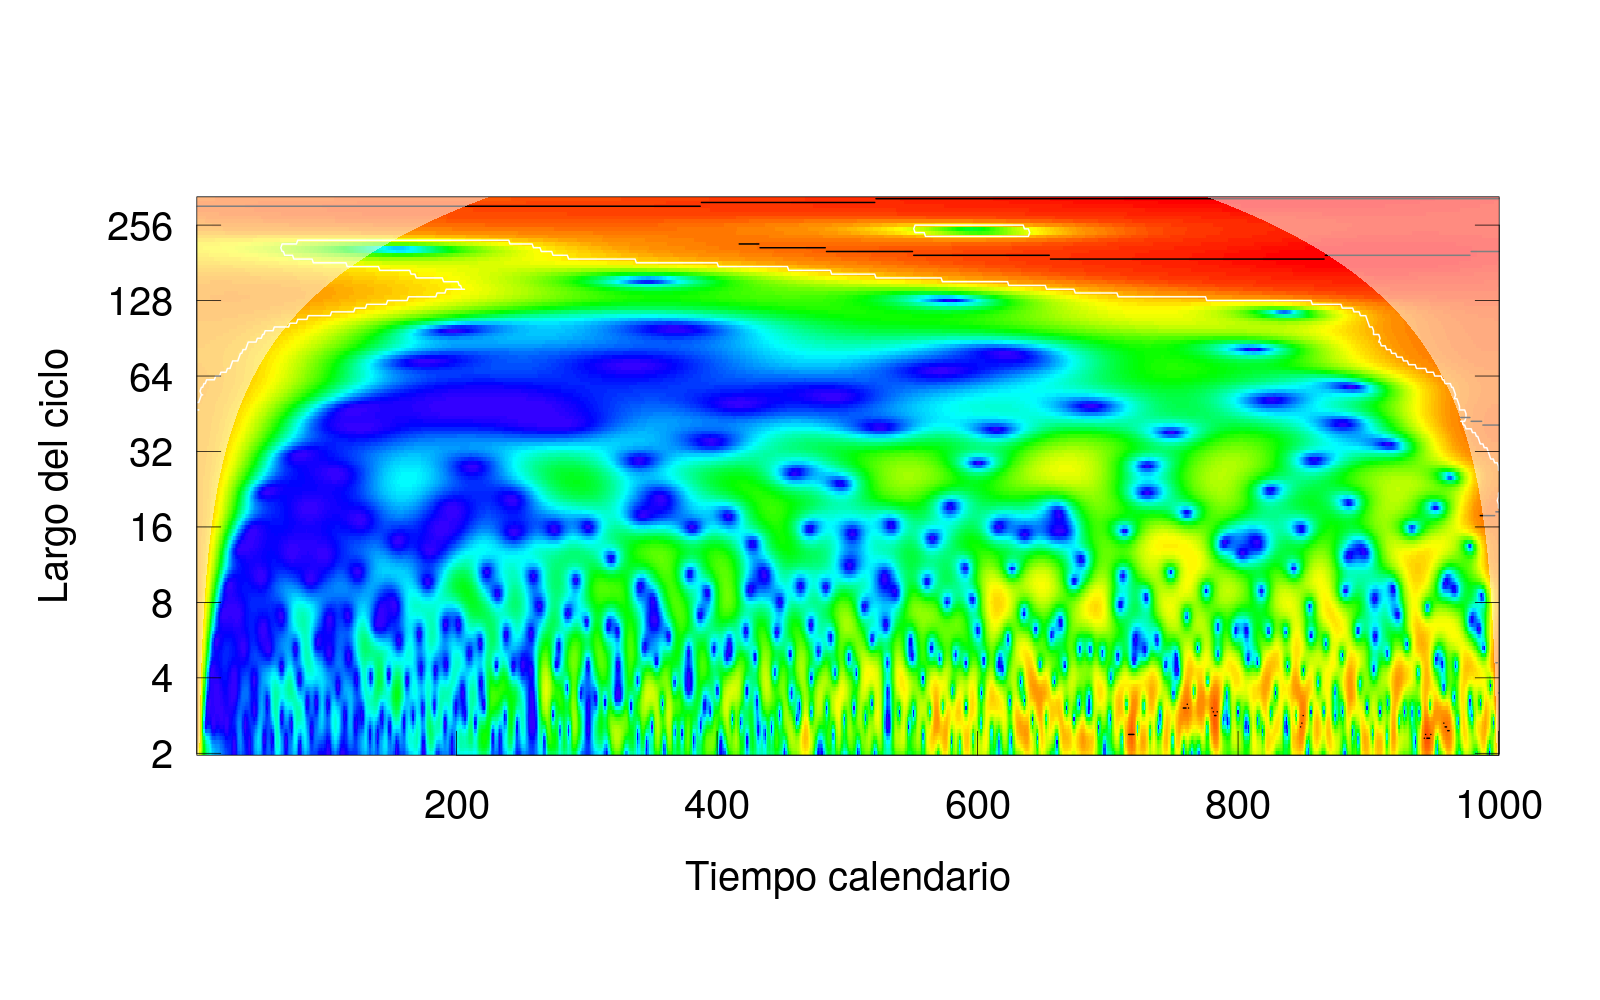
\includegraphics[width=0.49\linewidth]{espectograma_teorico_tendencia.png}}
	    \vspace{0.00mm}
	\subfigure[ciclo de 3 años]{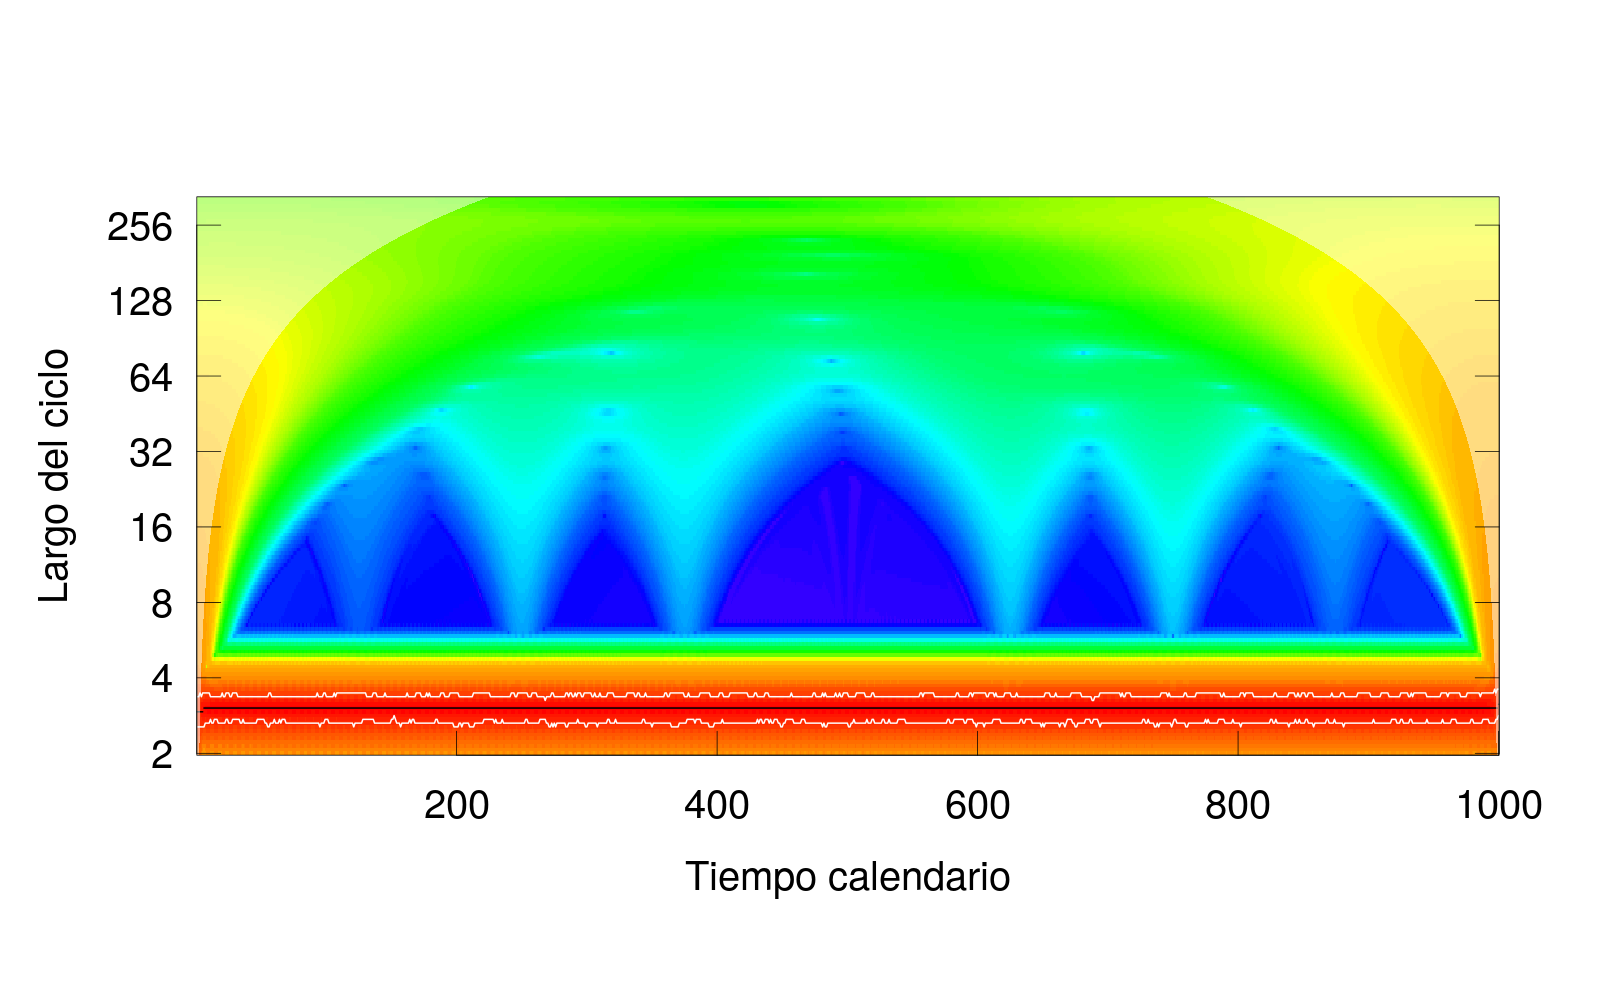
\includegraphics[width=0.49\linewidth]{espectograma_teorico_ciclo_3.png}}
	    \vspace{0.00mm}
	\subfigure[ciclo de 10 años]{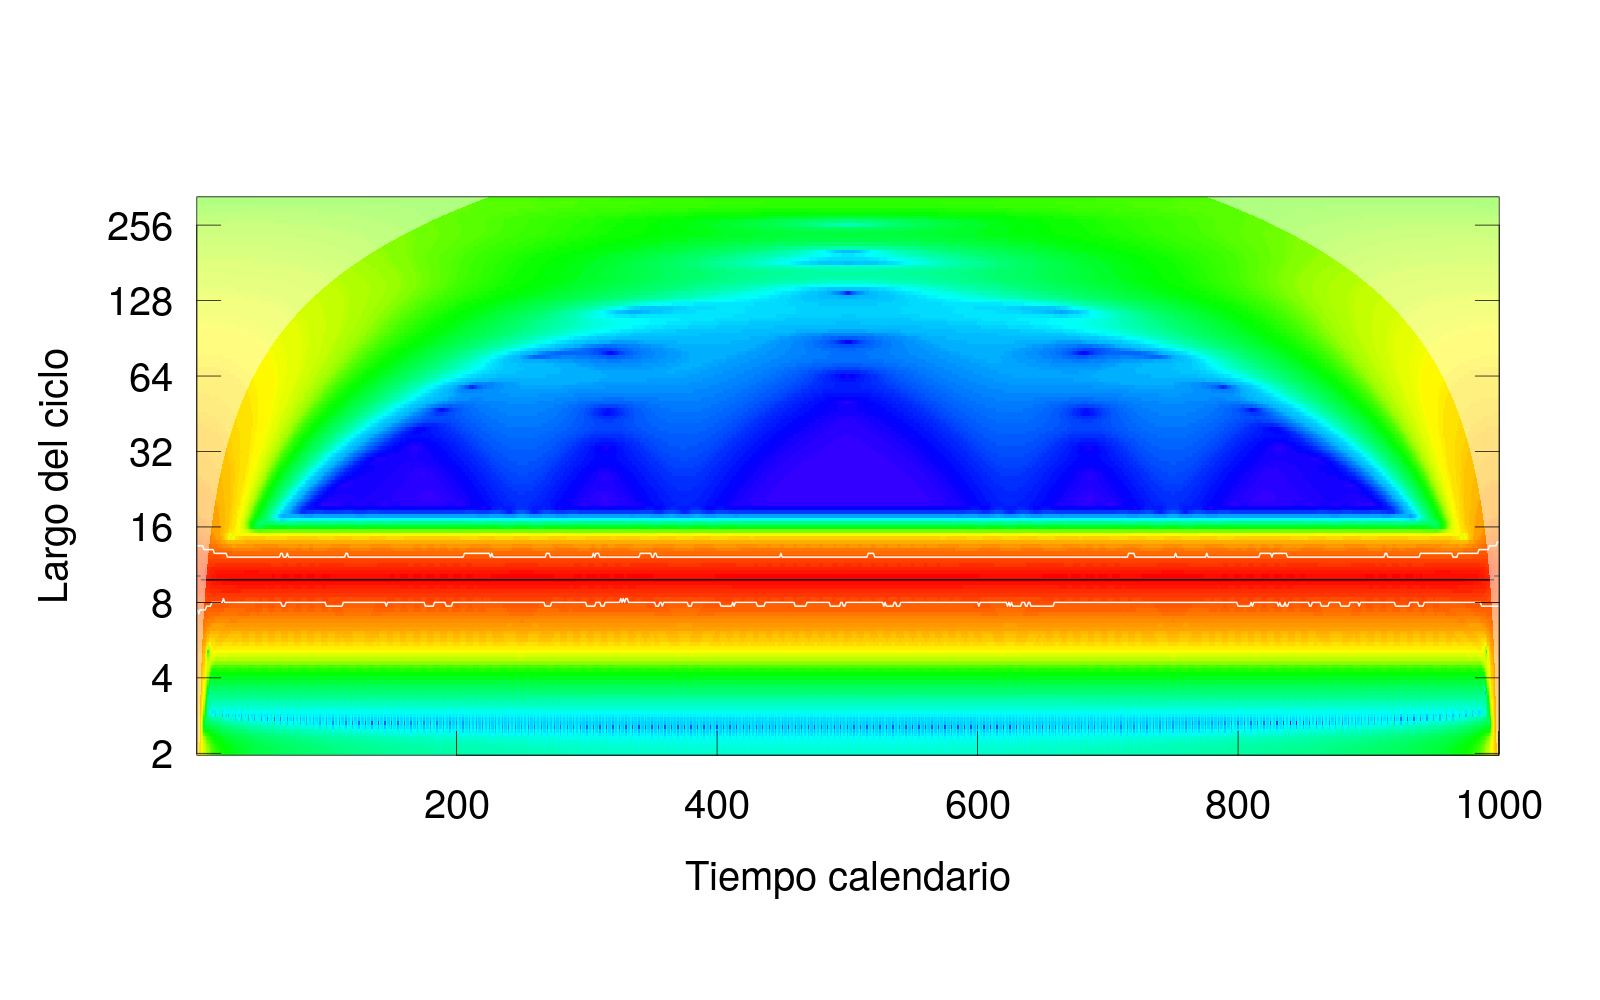
\includegraphics[width=0.49\linewidth]{espectograma_teorico_ciclo_10.png}}
	    \vspace{0.00mm}
	\subfigure[ciclo de 50 años]{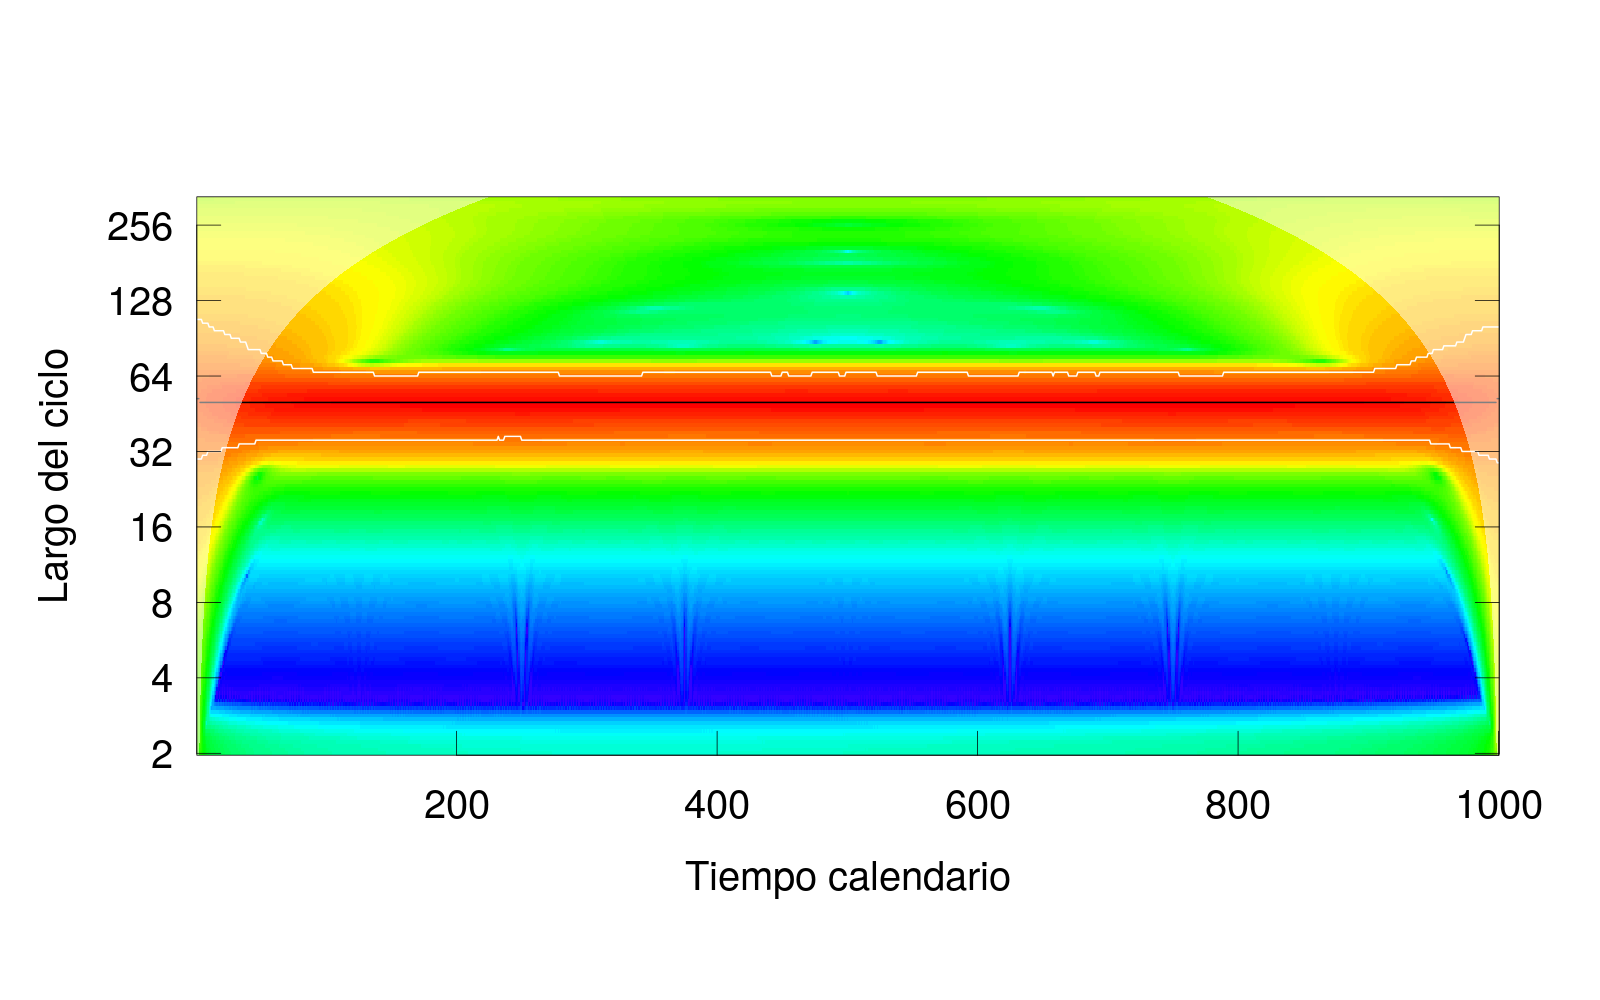
\includegraphics[width=0.49\linewidth]{espectograma_teorico_ciclo_50.png}}
	    \vspace{0.00mm}
	\subfigure[ruido normal]{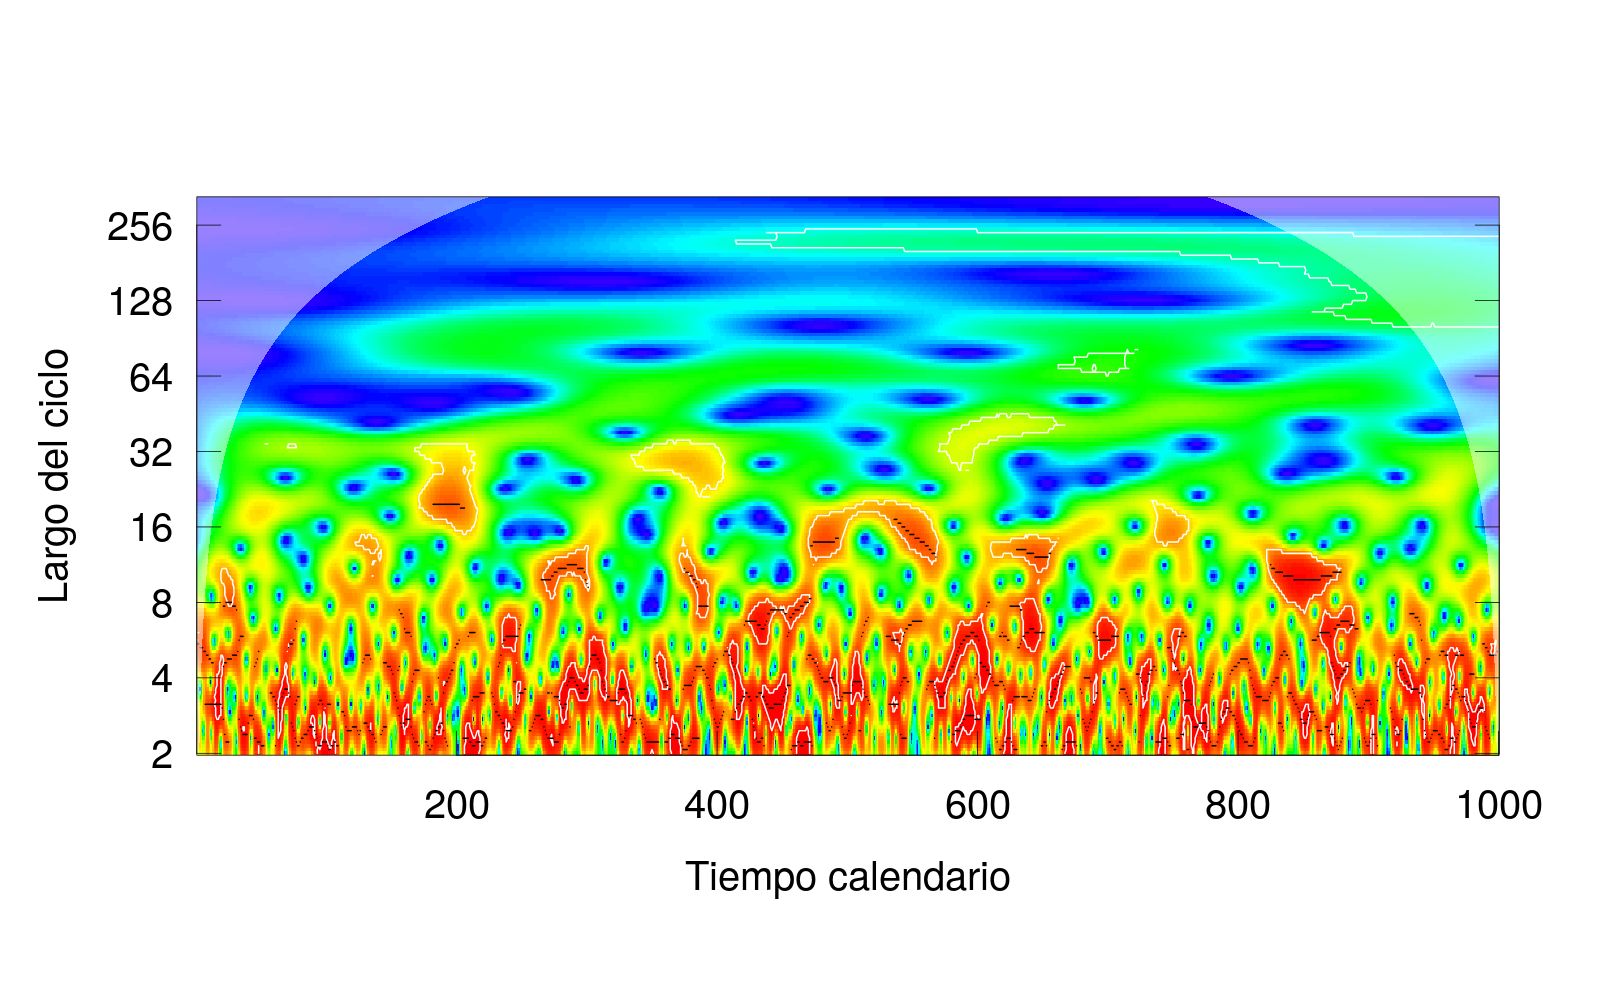
\includegraphics[width=0.49\linewidth]{espectograma_teorico_ruido.png}}
	    \vspace{0.00mm}
	\subfigure[composición de series]{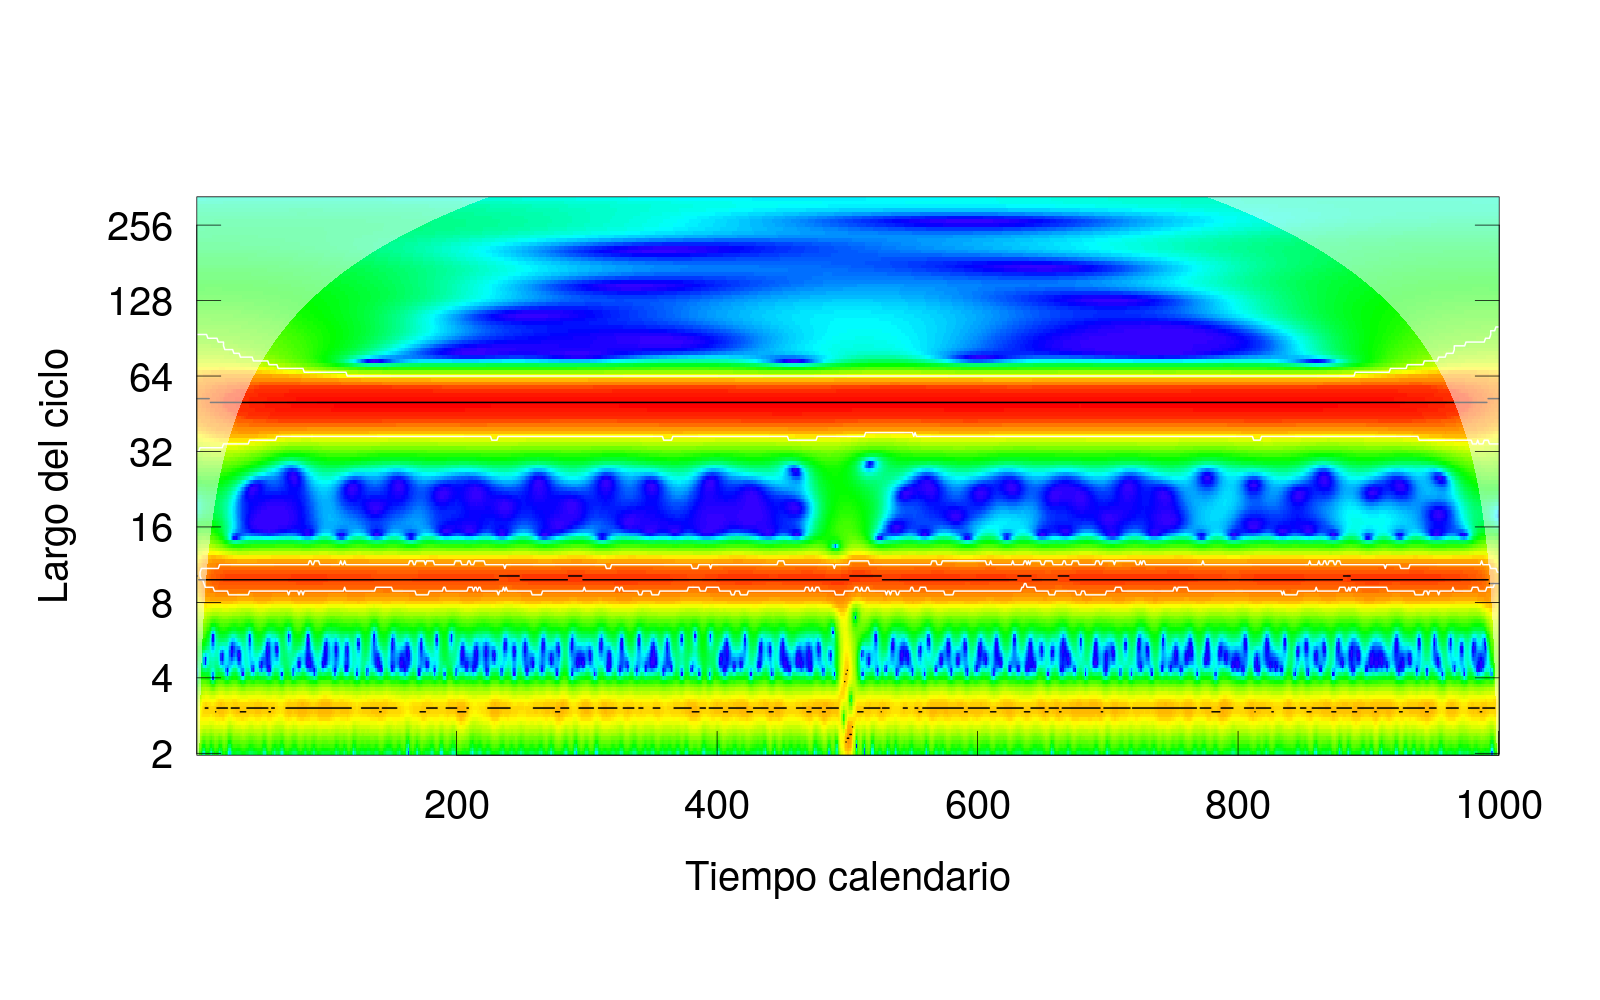
\includegraphics[width=0.75\linewidth]{espectograma_teorico_composicion_series.png}}
	\caption{Espectogramas teóricos} \label{fig:espect_teo}
\end{figure}

Como se observa en la figura \ref{fig:espect_teo} el impulso se presenta como un ciclo de amplitud grande en todas las frecuencias, en el momento correspondiente al salto. La tendencia, por su parte, se presenta básicamente como ruido, dado que es estrictamente un comportamiento no cíclico. Sin embargo, presenta la particularidad de tomar valores de amplitud mayores hacia el final del período para frecuencias bajas, y valores de amplitud particularmente bajos en las frecuencias altas de los primeros momentos.

Los tres ciclos definidos marcan claramente una línea horizontal en el correspondiente período, que luego se diluye hacia las demás frecuencias. Finalmente, el ruido normal presenta un comportamiento muy particular, mostrando mayores amplitudes, de forma irregular, en las frecuencias altas, y homogeneizándose hacia un valor de amplitud baja en los ciclos más largos. Esto se debe a que el ruido normal se puede parecer a un ciclo de períodos muy cortos debido a una sucesión de subas y bajas, pero dado que es un proceso aleatorio, es cada vez más improbable que se asemeje a ciclos de períodos mayores, siendo que ello implicaría una mayor cantidad de sucesiones de subas y bajas consecutivas. A su vez, tanto en el espectograma del ruido normal como en el de la tendencia se puede apreciar como el gráfico pierde resolución para periodos más largos, como se mencionó anteriormente. 

Por último, en la composición de series se observa como los ciclos de mayor amplitud y frecuencia se expresan en la escala cromática de forma más nítida que los ciclos de menor amplitud y frecuencia. Es importante resaltar que la concordancia entre amplitud y frecuencia es producto de la forma en que construimos las series, dado que esperamos que los ciclos económicos más largos se correspondan también con movimientos de mayor amplitud.

Vale mencionar que la elección para el modelo teórico de estos tres niveles y amplitudes cíclicas no es arbitraria, sino que se corresponde a grandes rasgos con lo considerado por la literatura: \cite{kondratieff1979long} estudia las series largas, de unos 50 años, mientras que \cite{kuznets1930secular} propone movimientos seculares de entre 15 y 25 años. Finalmente el Real business cycle \citep{kydland1982time} considera un ciclo corto.



Con lo analizado de la figura \ref{fig:espect_teo} podemos observar los resultados de las series originales. En la figura \ref{fig:espect_PBI_a} se puede observar el espectograma correspondiente al PBI de Estados Unidos expresado en oro. Allí se marca claramente la diferencia en la serie antes y después del 1900, y en particular también se marca el quiebre estudiado de los años 70'. No obstante lo cual, para ese período se observan 3 frecuencias donde se registra un comportamiento cíclico, en los períodos aproximados de 8 y 50 años, y un ciclo diferenciado de este último, de aproximadamente 30 años. Dada la heterocedasticidad de las series, en \ref{fig:espect_PBI_b} se propone el espectograma de la misma serie tomada en logaritmo de base 10. De esta forma lo que se observa es que el ciclo de 50 años se extiende más allá en el tiempo, hasta mediados del Siglo XIX. Por su parte, aparece brevemente un ciclo más corto, de aproximadamente tres años, en la década del 70.

\begin{figure}[H]
	\centering
	\subfigure[PBI]{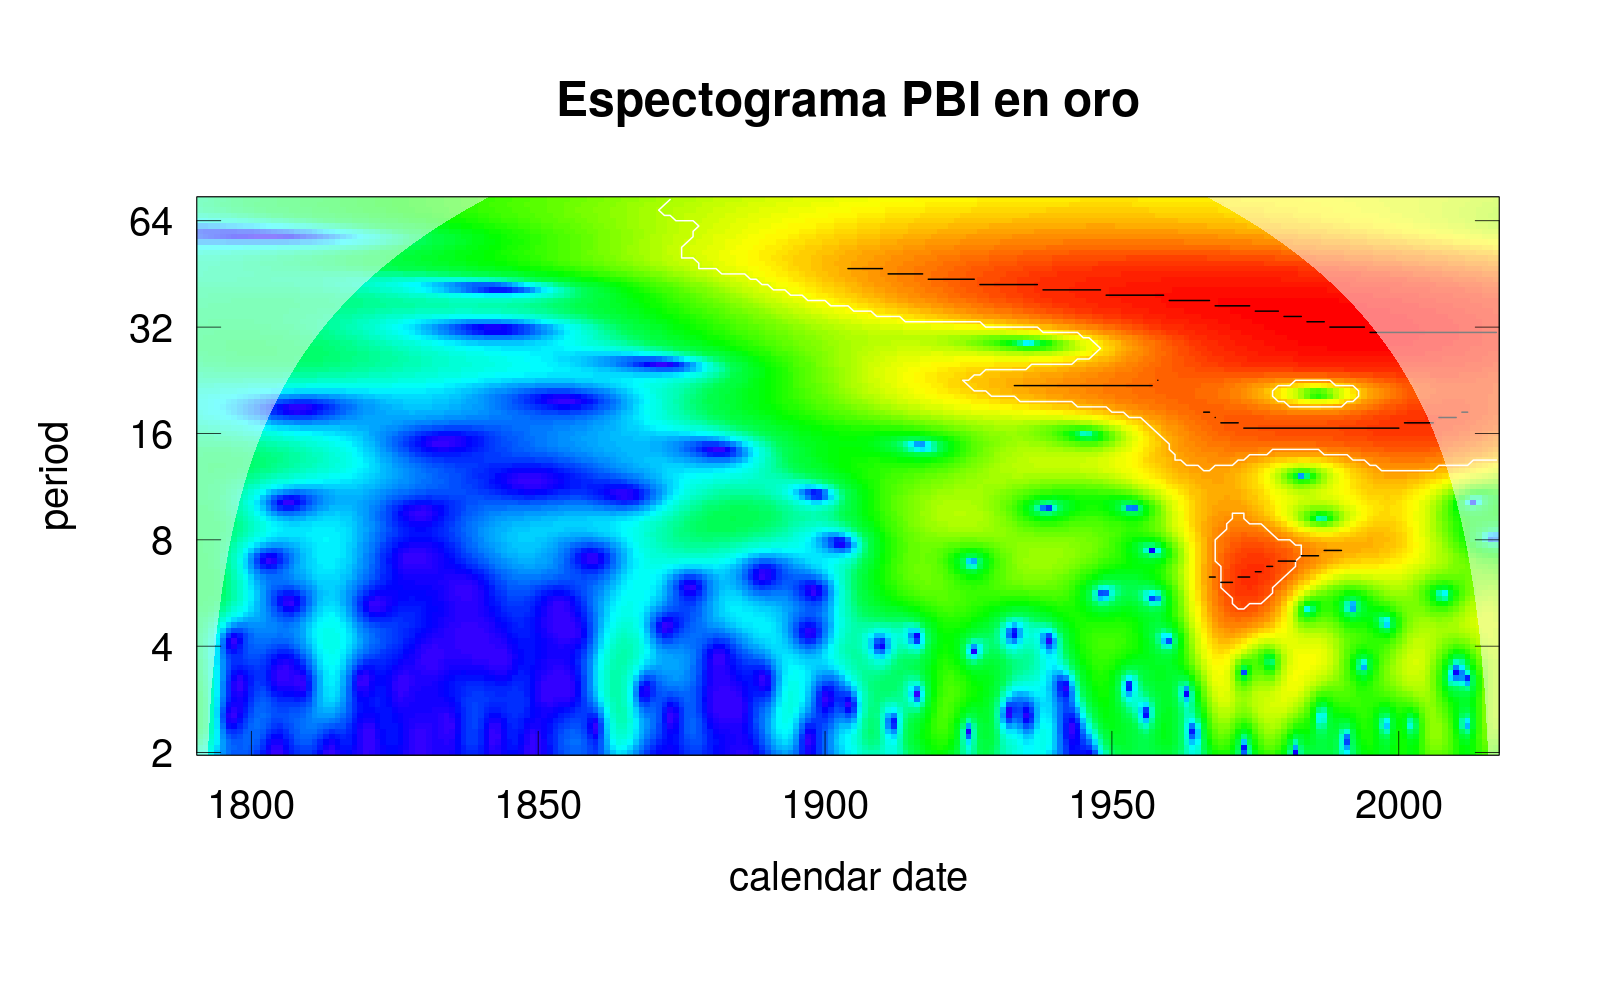
\includegraphics[width=0.75\linewidth]{espectograma_gdp.png}
	\label{fig:espect_PBI_a}}
	\subfigure[$log(PBI)$]{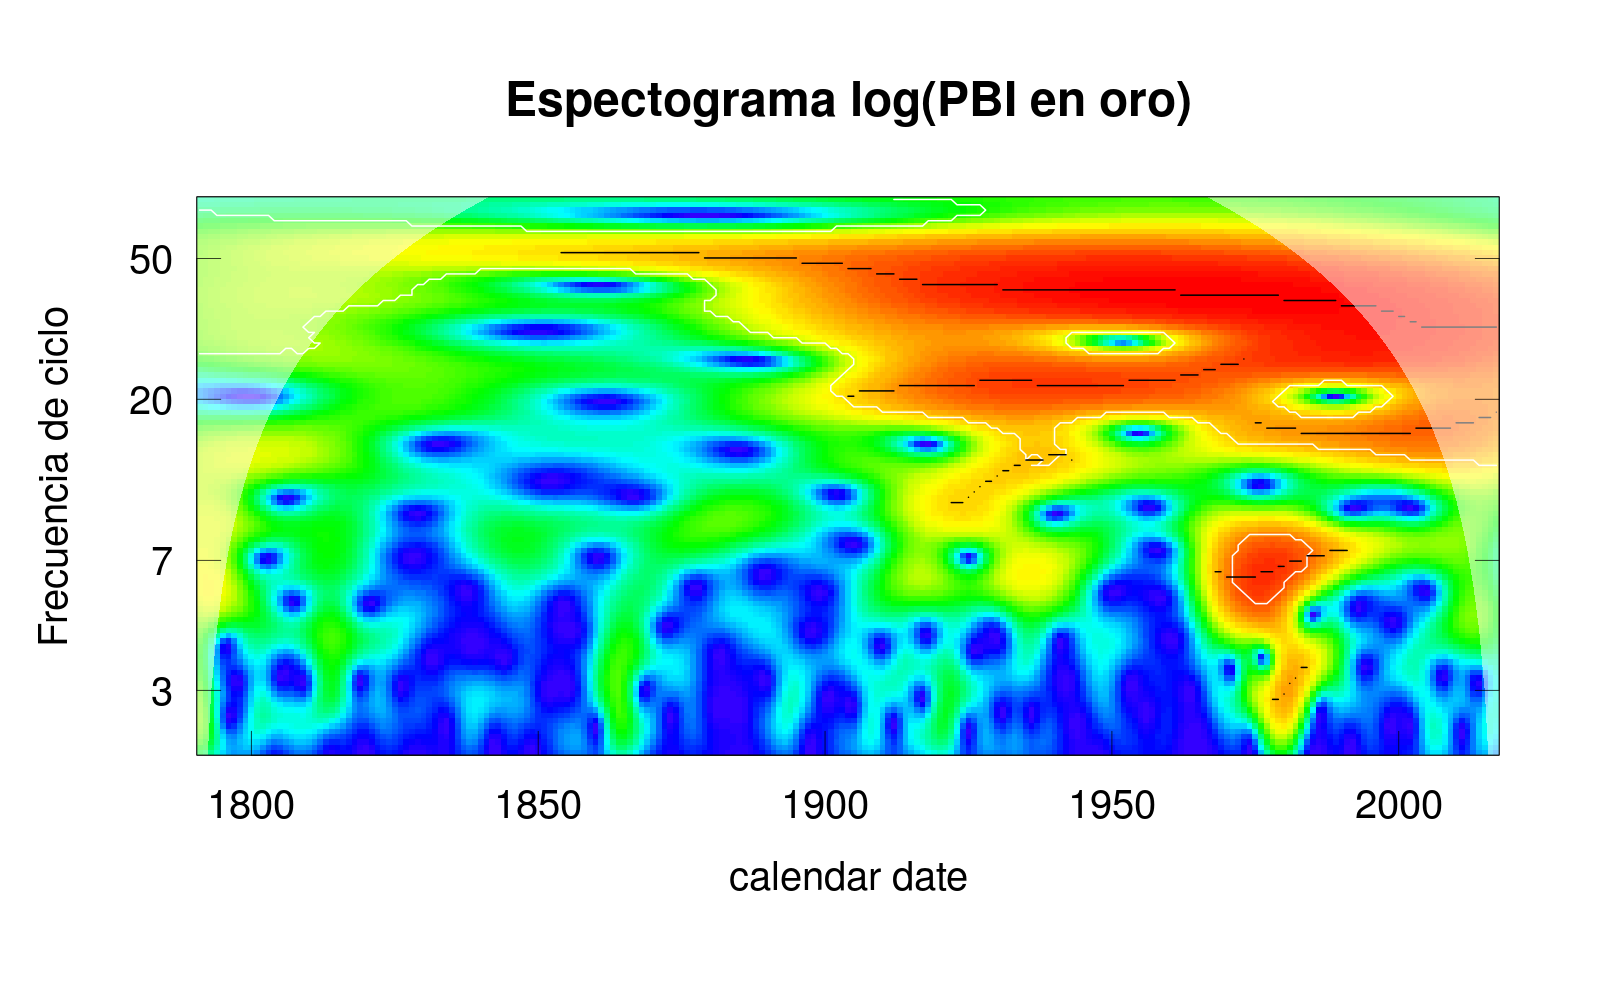
\includegraphics[width=0.75\linewidth]{espectograma_log_gdp.png}
	\label{fig:espect_PBI_b}}
	\caption{Espectograma PBI en oro} \label{fig:espect_PBI}
\end{figure}

las figuras \ref{fig:espect_wg} muestran los espectogramas de la serie del salario expresado en oro \ref{fig:espect_wg_a} y el mismo tomado en logaritmo en \ref{fig:espect_wg_b}. Para esta serie nuevamente se observa un ciclo largo bien definido en torno a los 50 años, especialmente si se observa la serie tomada en base logarítmica. Este ciclo largo parece oscilar entre las frecuencias de $1/32$ y $1/64$, cayendo en el tiempo. Por su parte, se delimita un segundo ciclo, en torno a los 16 años de extensión, y finalmente un ciclo corto de entre 6 y 8 años.  Al tomar la escala logarítmica, también aparece un ciclo de mayor frecuencia, de unos 3 años de duración. En consecuencia, ambas series parecen arrojar resultados en concordancia, sean o no tomadas en logaritmo. 

\begin{figure}[H]
	\centering
	\subfigure[Salario]{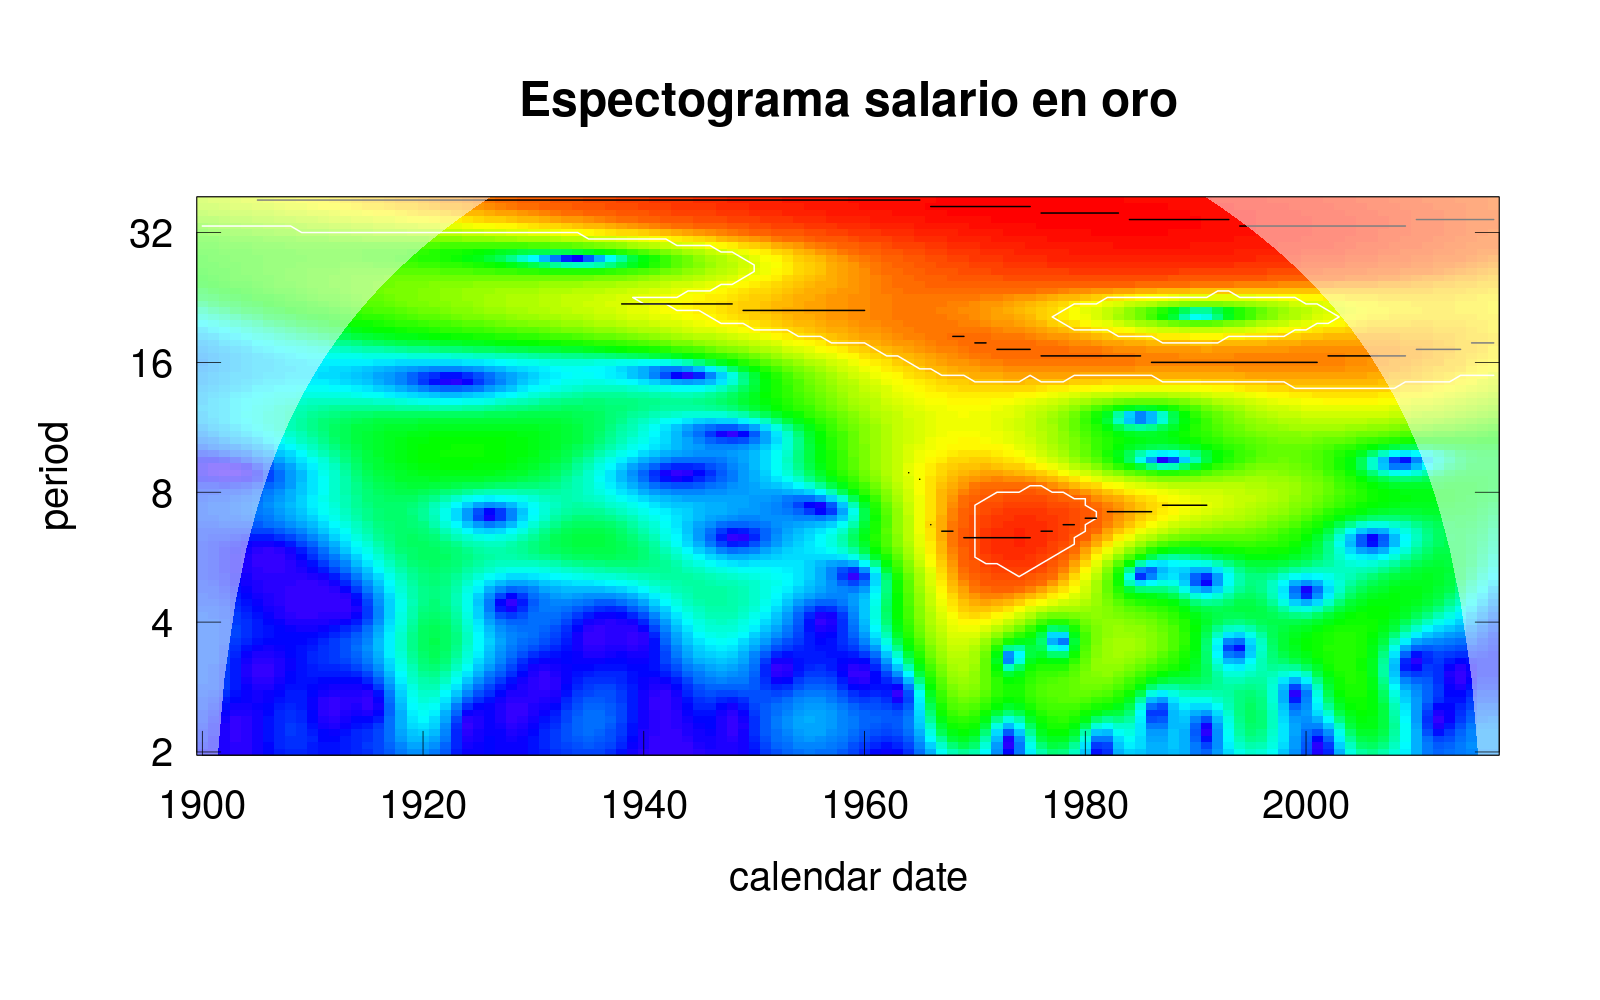
\includegraphics[width=0.75\linewidth]{espectograma_wg.png}
	\label{fig:espect_wg_a}}
	\subfigure[$log(Salario)$]{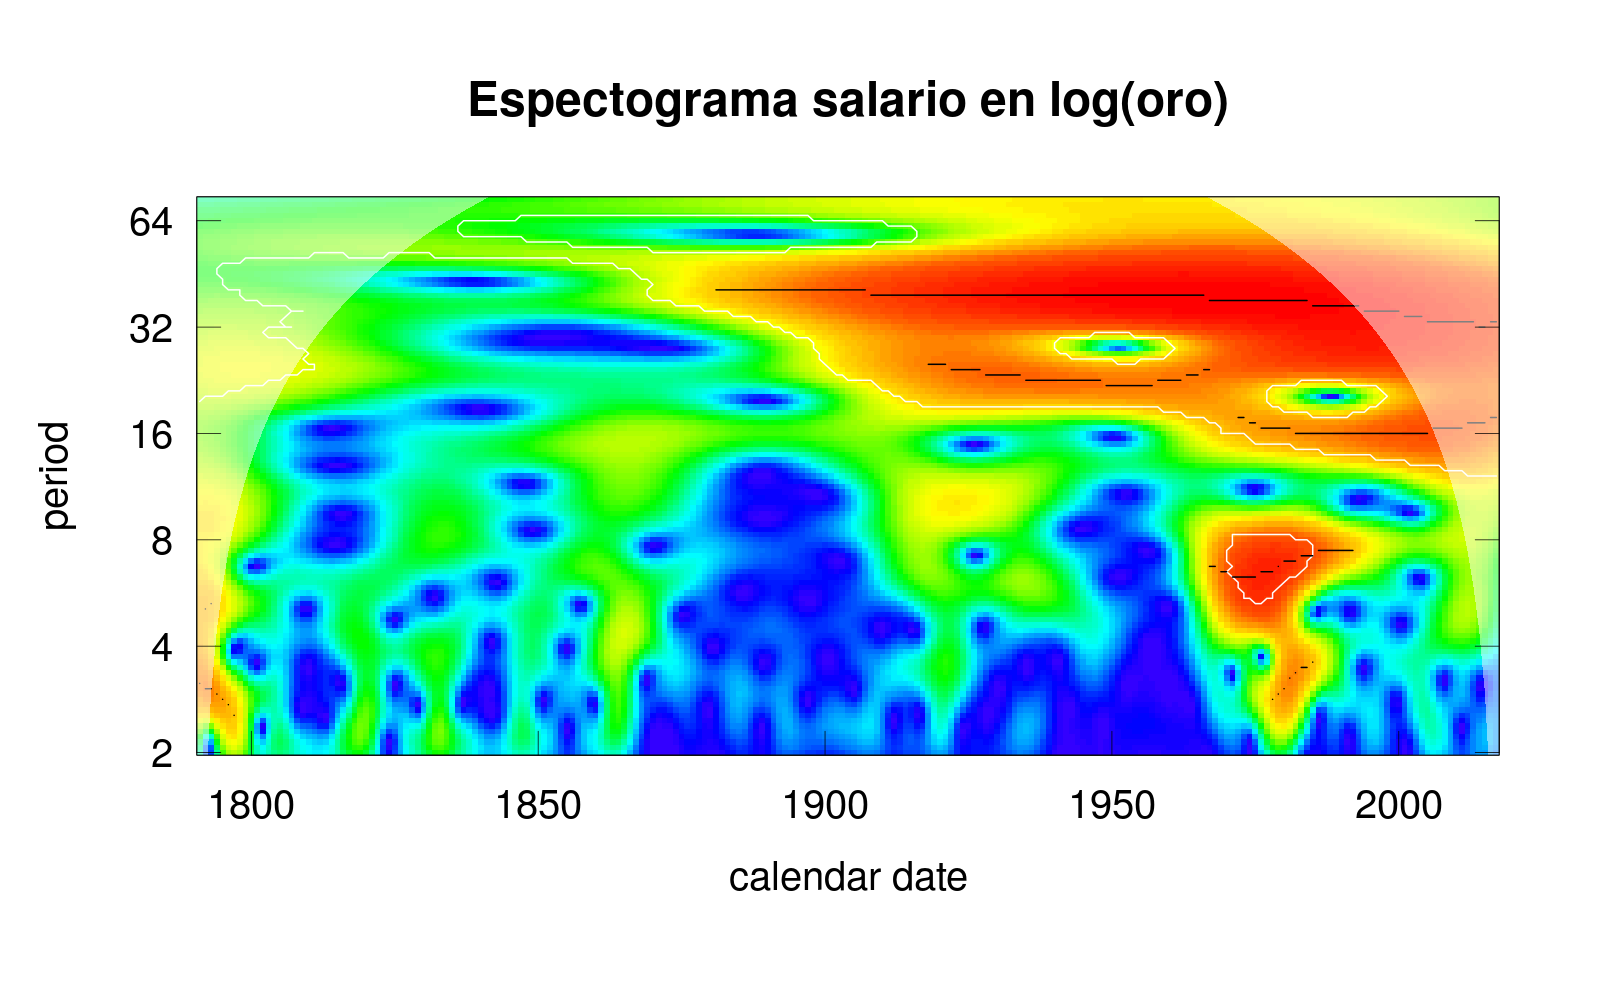
\includegraphics[width=0.75\linewidth]{espectograma_log_wg.png}
	\label{fig:espect_wg_b}}
	\caption{Espectograma Salario en oro} \label{fig:espect_wg}
\end{figure}


En la figura \ref{fig:espect_uk} se muestra la serie del PBI expresado en oro para el Reino Unido entre 1700 y 1900. Al igual que en las series anteriores se expresa la serie sin transformaciones adicionales en \ref{fig:espect_uk_a} y expresada en logaritmo en \ref{fig:espect_uk_b}. A diferencia de la serie de Estados Unidos, aquí se puede observar con más claridad el ciclo corto, en torno a los 10 años. 


\begin{figure}[H]
	\centering
	\subfigure[PBI UK]{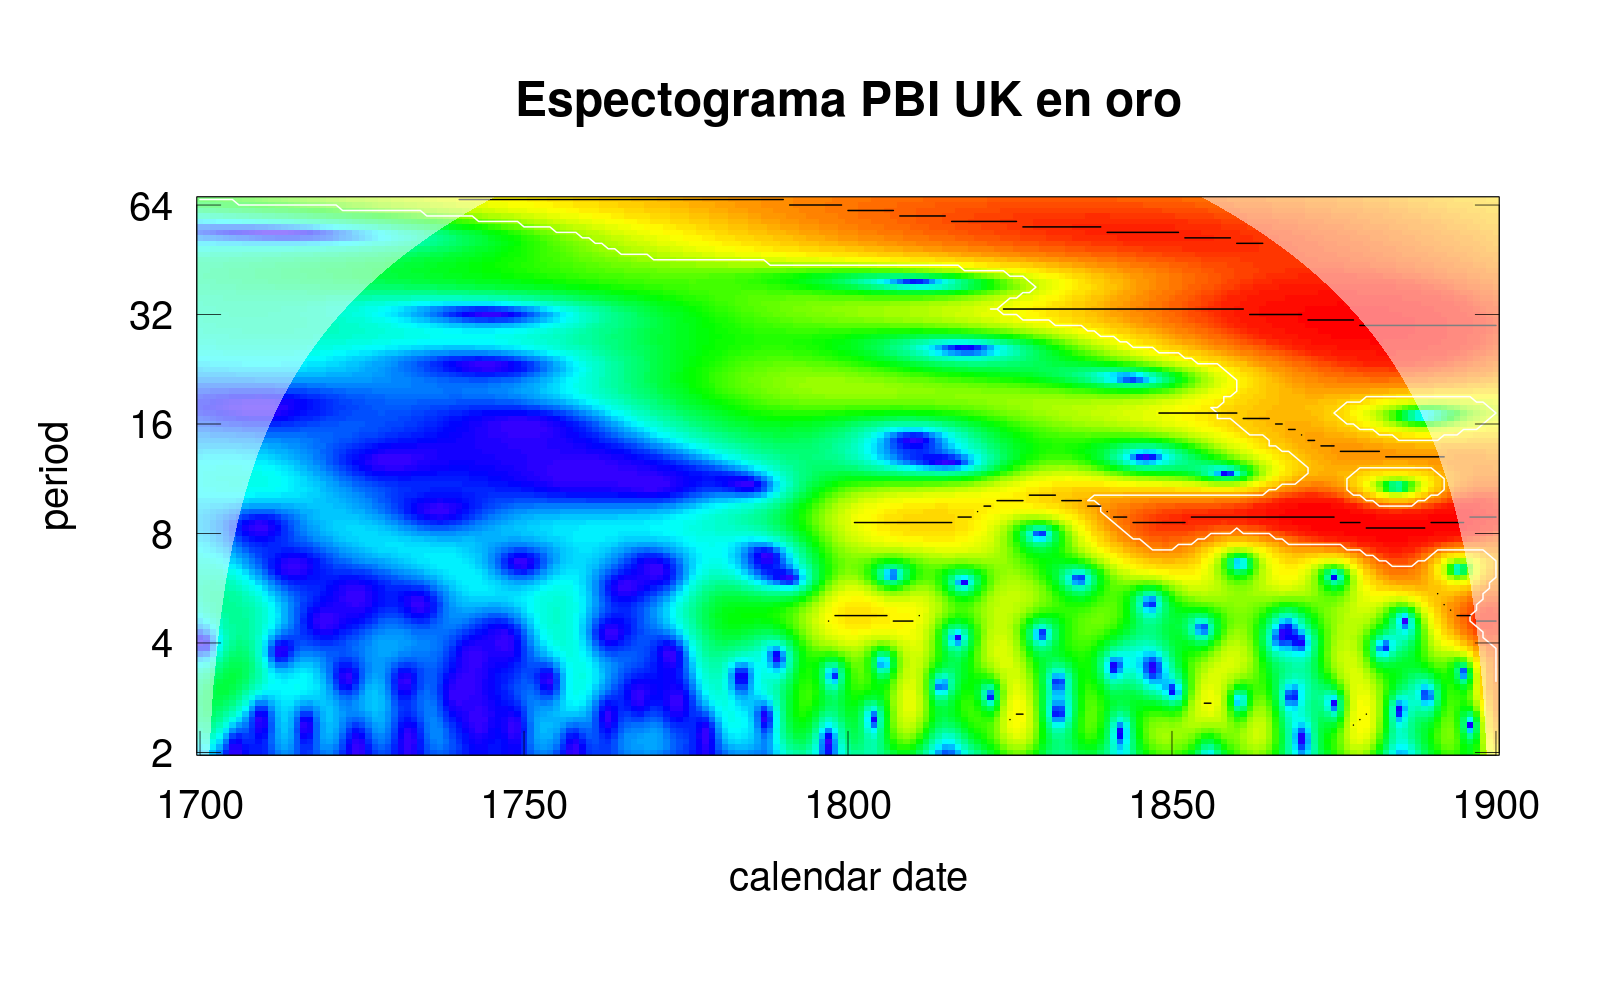
\includegraphics[width=0.75\linewidth]{espectograma_gdp_uk.png}
		\label{fig:espect_uk_a}}
	\subfigure[$log$(PBI UK)]{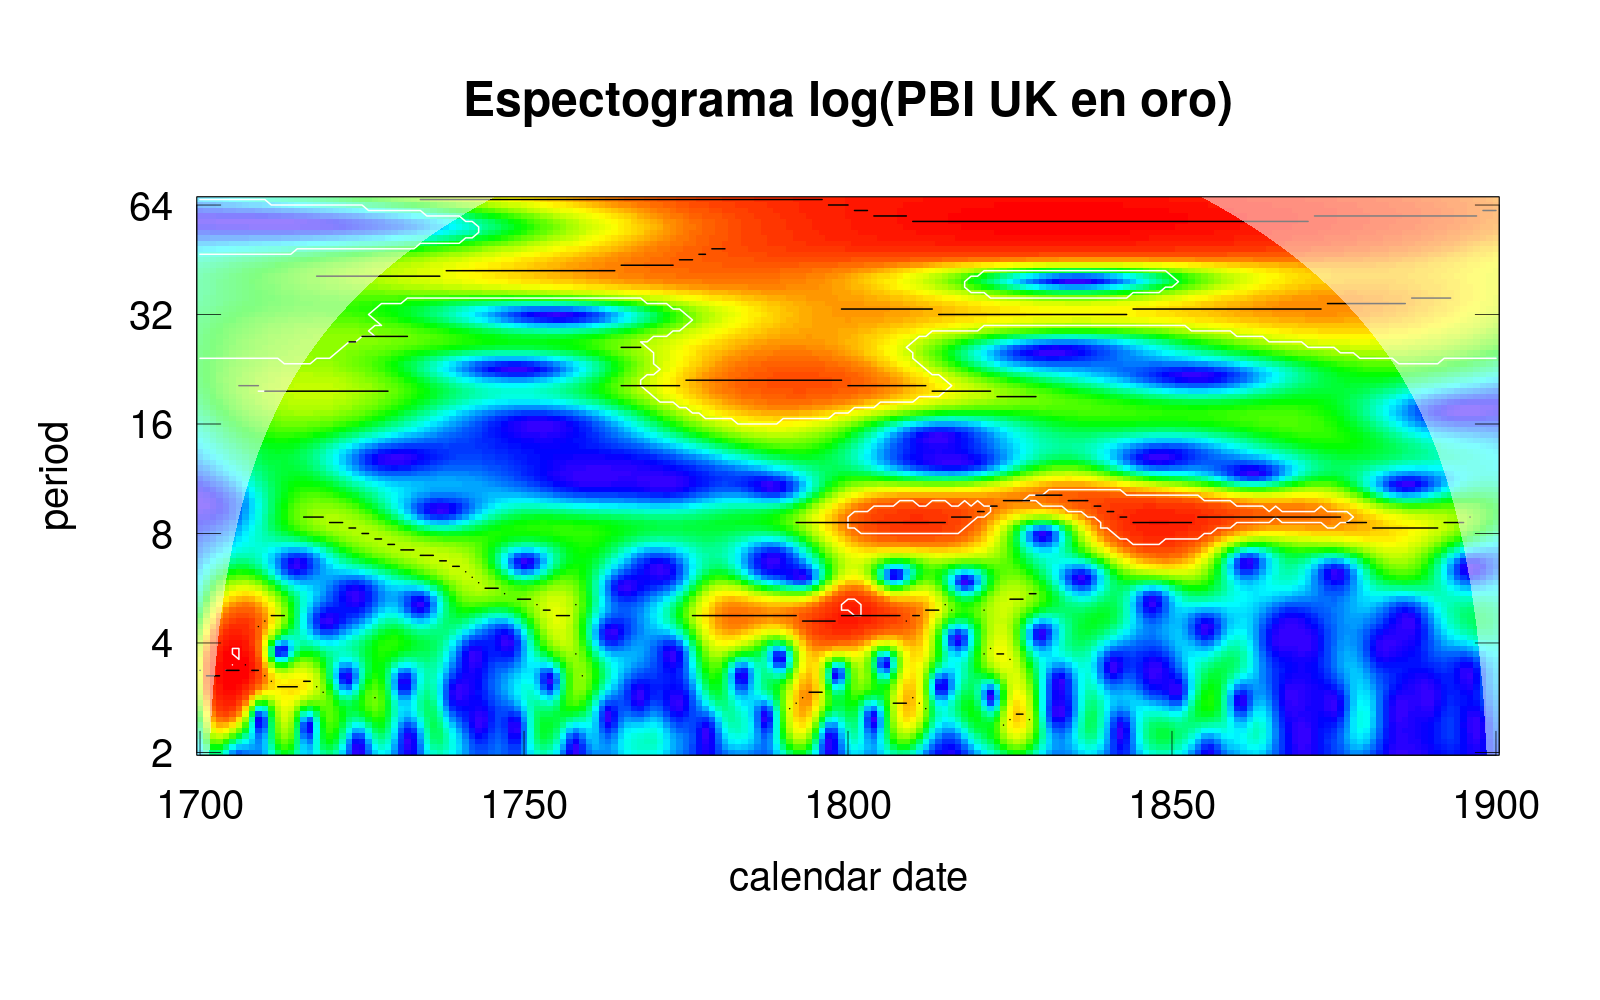
\includegraphics[width=0.75\linewidth]{espectograma_log_gdp_uk.png}
		\label{fig:espect_uk_b}}
	\caption{Espectograma PBI Reino Unido} \label{fig:espect_uk}
\end{figure}

A su vez, otra diferencia que destaca es que en las figuras de Reino Unido el efecto de la transformación logarítmica es mayor que en las series anteriores. De esta forma, en \ref{fig:espect_uk_b} se puede observar una multiplicidad de ciclos que destacan como influyentes. En particular, el más corto pareciera estar en torno a los cuatro años de duración, especialmente presente al principio de la serie y en el entorno del 1800. Luego destaca el ciclo en torno a los 8 años de duración, asociado en la descripción realizada en el Análisis Exploratorio de Datos con lo que se marcaba como un ciclo de 10 años. De mayor extensión temporal se intercala un ciclo en torno a los 20 años, al principio de la serie y en el entorno del 1800, junto con un ciclo de 30-35 años en los períodos restantes. Finalmente, vuelve a registrarse un ciclo largo, en torno a los  64 años de extensión. 

Es importante registrar el efecto que produce la tendencia de la serie sobre los espectogramas. En la figura \ref{fig:uk_gdp} se observaba un fuerte efecto tendencial del producto expresado en oro para el Reino Unido durante los siglos XVIII y XIX. Dicha tendencia no pareciera ser lineal y por lo tanto resulta de interés analizar las posibles distorsiones que esto puede generar sobre los espectogramas. en la figura \ref{fig:tendencias} se puede observar el PBI del Reino Unido en oro, junto con un suavizado lineal mediante un modelo de regresiones locales \citep{Shyu1992}, y la serie resultante de eliminar dicha tendencia. 

En efecto, en la figura \ref{fig:espectograma_gdp_uk_Tend} se observa el espectograma de la tendencia calculada sobre la serie. Allí se destaca el período en torno a los cincuenta años, lo que pareciera indicar que aquello descripto hasta este momento es un simple efecto tendencial oculto en los espectogramas. Sin embargo, en la figura \ref{fig:espectograma_sin_tend} se observa el espectograma de la serie del producto para el Reino Unido, expresado en oro, pero luego de restar la tendencia de la serie. Se puede apreciar que dicho espectograma es casi idéntico al visto anteriormente en la figura \ref{fig:espect_uk_a}. Esto quiere decir que la técnica de wavelets no se ve afectada por la tendencia subyacente de las series analizadas.

\begin{figure}[H]
	\centering
	\subfigure[]{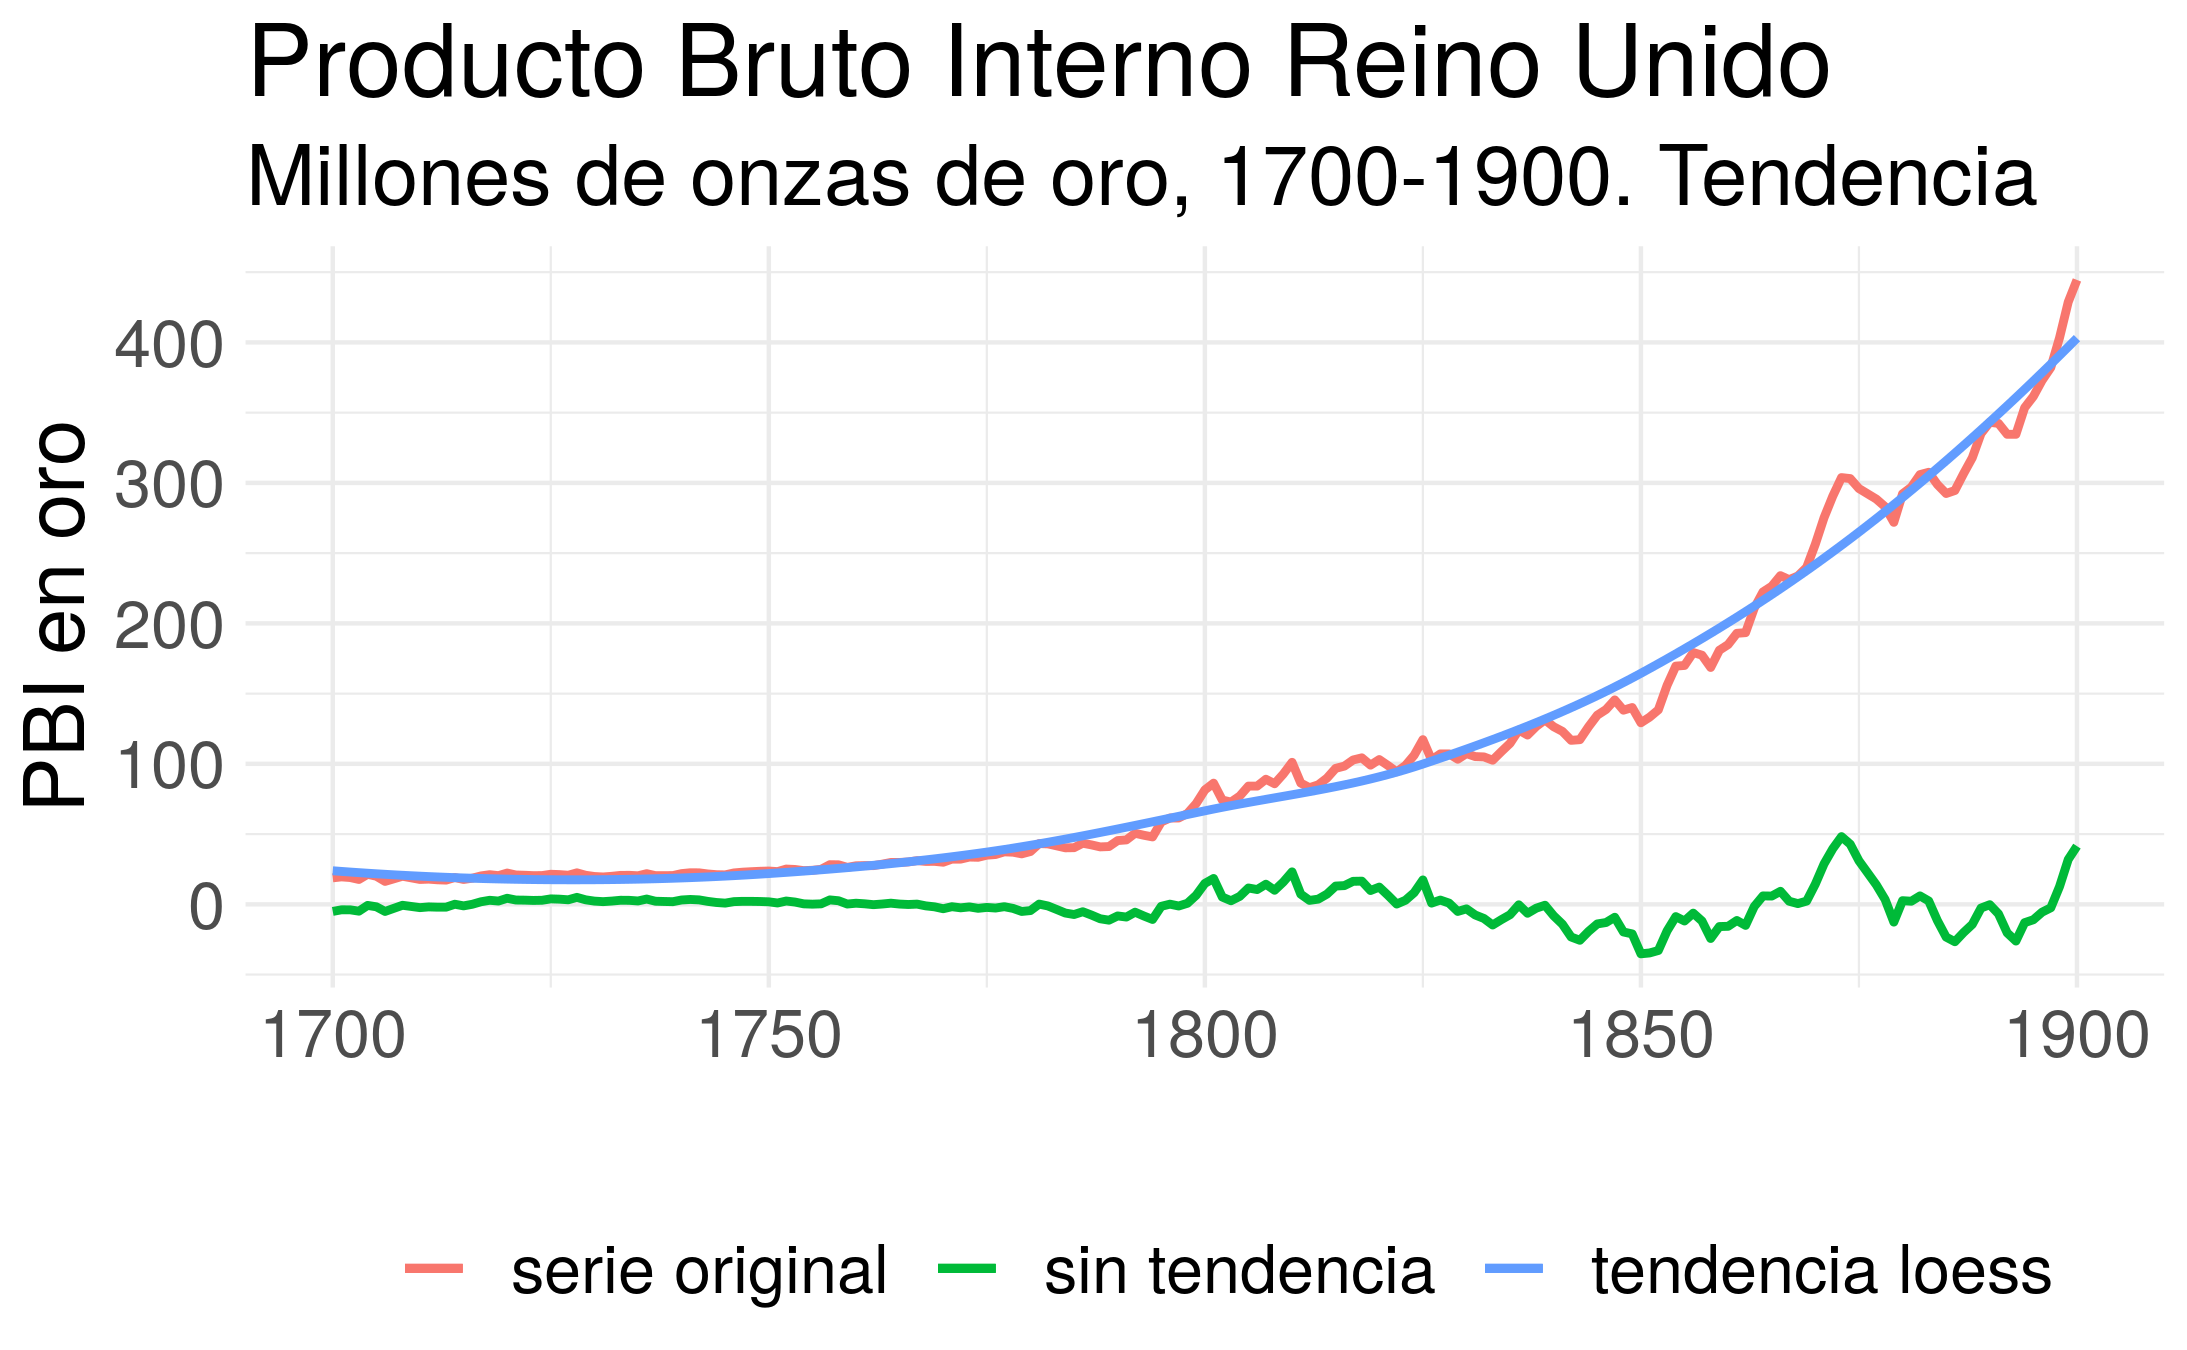
\includegraphics[width=0.75\linewidth]{pbi_uk_tendencias.png}
		\label{fig:tendencias}}
	\subfigure[]{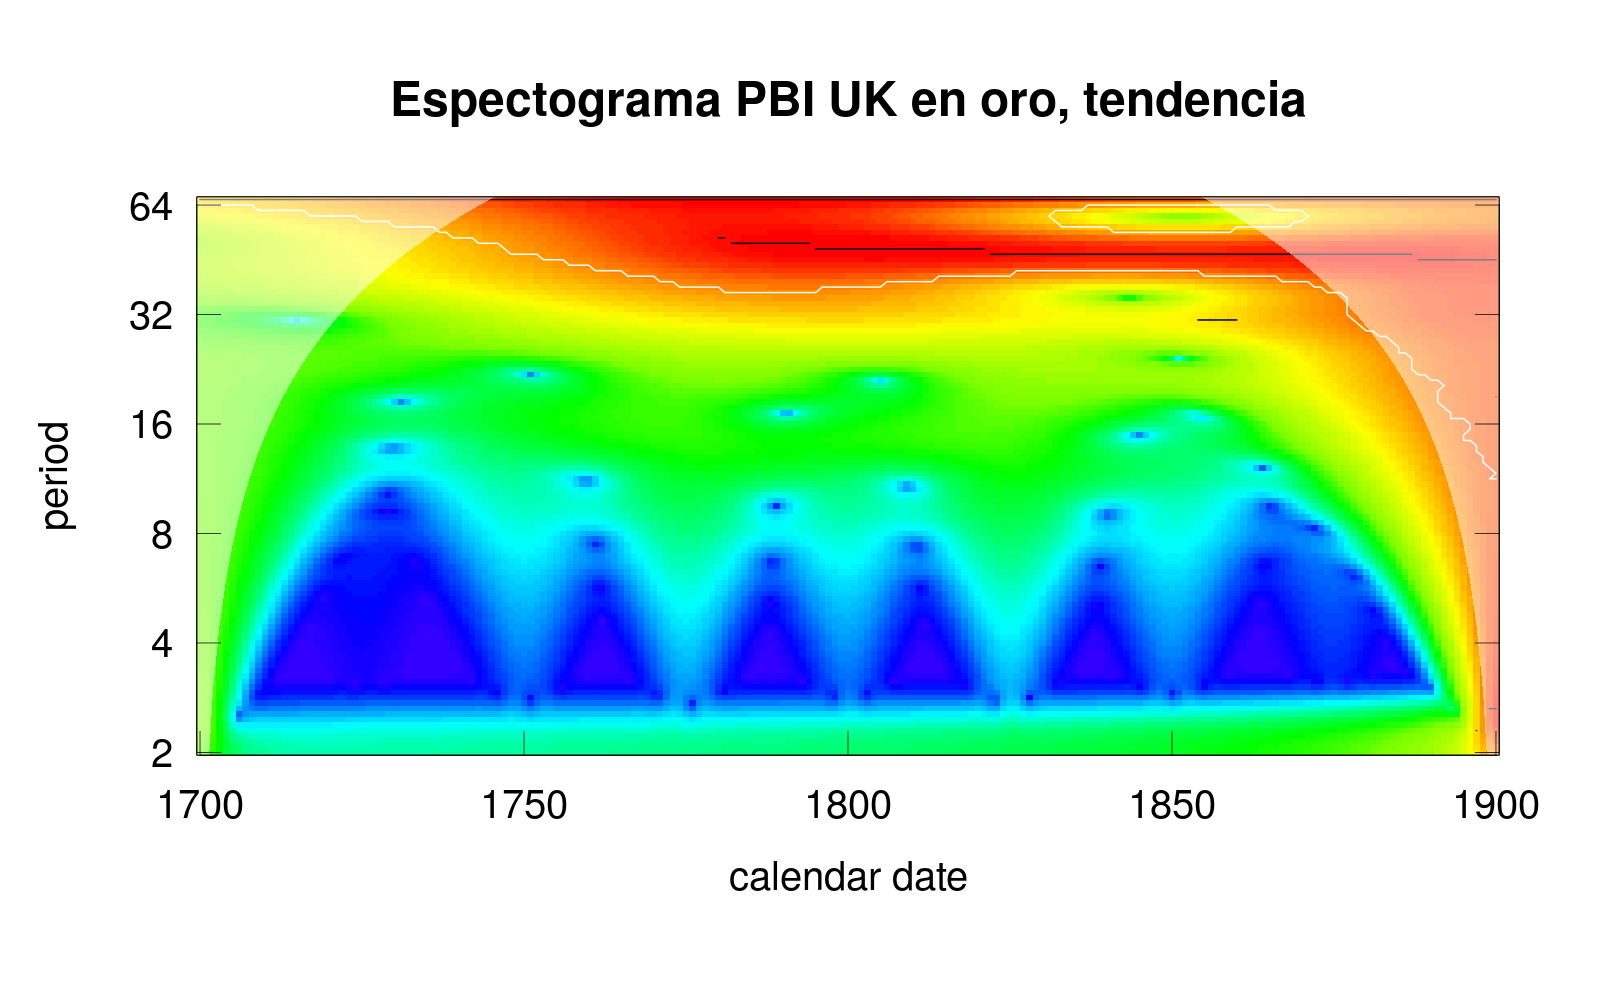
\includegraphics[width=0.48\linewidth]{espectograma_gdp_uk_Tend.png}
		\label{fig:espectograma_gdp_uk_Tend}}
	\subfigure[]{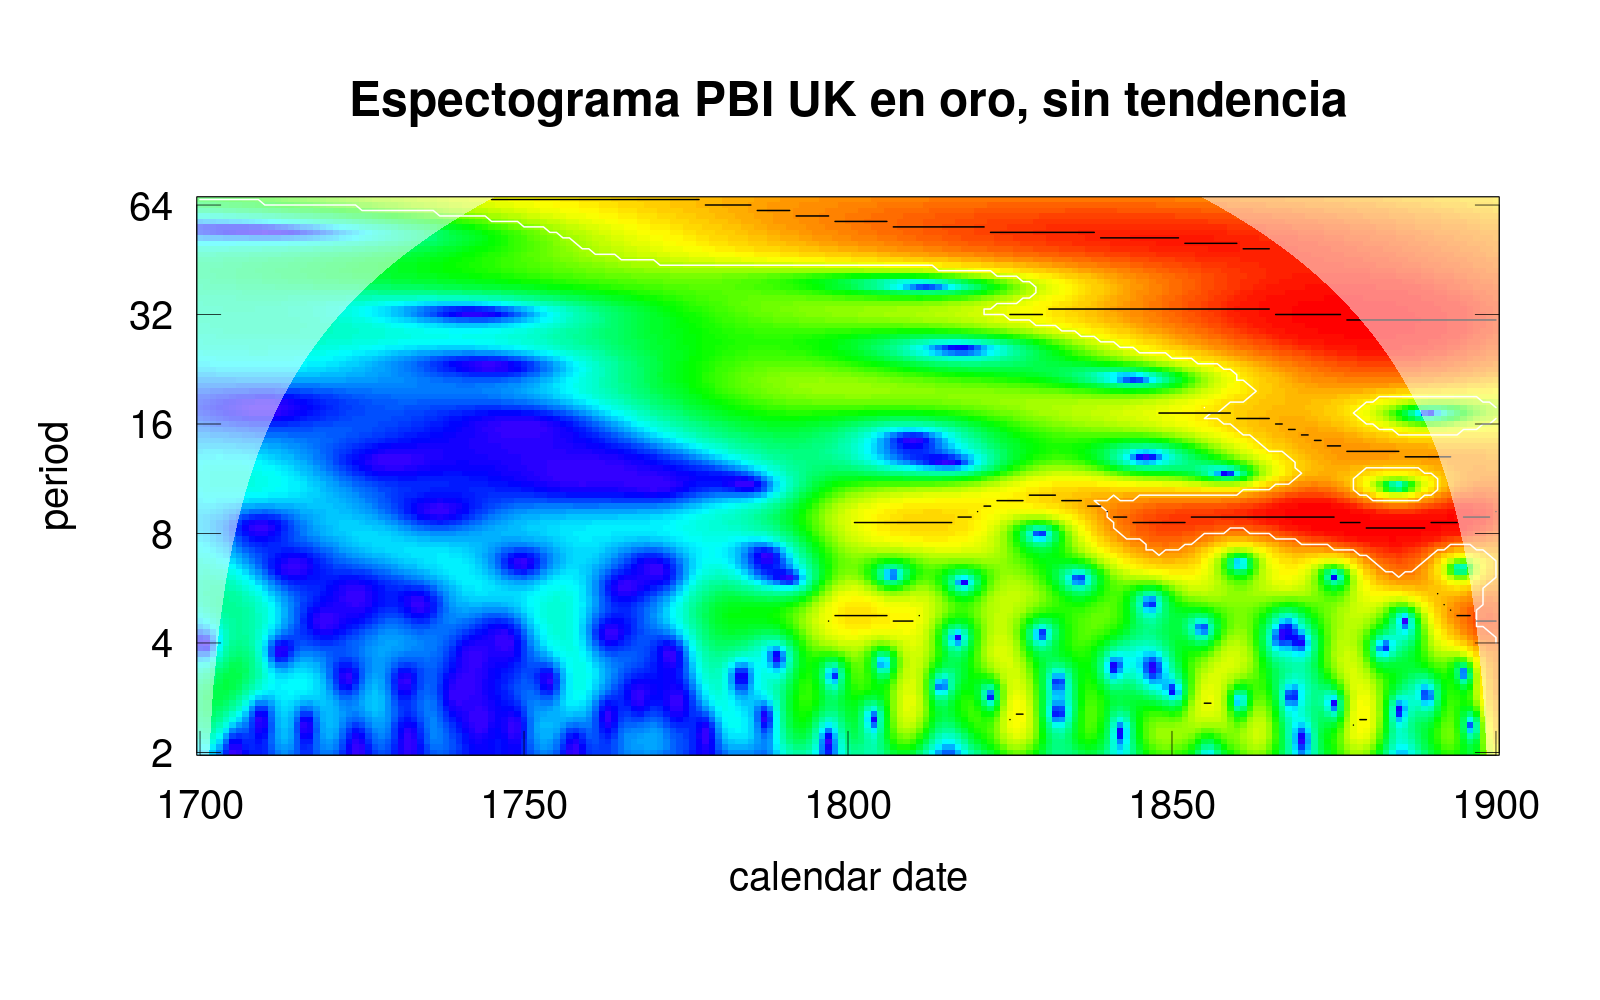
\includegraphics[width=0.48\linewidth]{espectograma_gdp_uk_sinTend.png}
		\label{fig:espectograma_sin_tend}}
	\caption{Efecto tendencia} \label{fig:espect_tendencias}

\end{figure}





\section{Conclusiones}

En el presente trabajo se realizó un recorrido por las principales aproximaciones teóricas respecto al ciclo económico, y se planteó la importancia de un análisis empírico respecto a dicho fenómeno. Para ello, se utilizaron las series de PBI y Salario de Estados Unidos entre 1790 y 2017, expresadas en oro, por los efectos distorsivos que podría generar dicha variable. También se utilizó la serie del PBI para el Reino Unido, entre 1700 y 1900

En el Análisis Exploratorio de Datos se encontró una fuerte correspondencia entre los quiebres de estas series, y las crisis conocidas por la historiografía económica, así como un movimiento oscilatorio aparente que pareciera corresponderse con las ondas largas de Kondratieff para el siglo XX, junto con las particularidades que exhiben las distintas series según el período de tiempo considerado. Por su parte, el siglo XIX en Reino Unido pareciera resaltar las crisis en torno a los 10 años de duración.

Luego se realizó un análisis en base a \textit{Wavelets}, una herramienta poco utilizada en el análisis económico de las series de tiempo, pero con la cual se puede visualizar la correspondencia de las series económicas con los ciclos a diferentes extensiones. Los resultados de esta técnica muestran la existencia de tres ciclos bien definidos a distintas frecuencias, los cuales se corresponden con las hipótesis estudiadas sobre la existencia de un ciclo corto, uno medio y uno largo. También es importante mencionar que esta herramienta pierde resolución en ciclos de períodos muy largos, y que entre las distintas series analizadas existen ciertas diferencias de nivel en los mismos. En este sentido, la herramienta vista no permite definir con exactitud la extensión temporal de cada uno de los ciclos, sino que simplemente demuestra su existencia.

Es importante remarcar que el objetivo del presente trabajo es buscar evidencia empírica respecto de la frecuencia y amplitud del comportamiento cíclico de la economía. Se toma las series de salario y PBI por ser buenos aproximadores de movimiento económico general, pero no son los únicos. A su vez, como las estadísticas tienen una base nacional, el PBI siempre es de un país en particular, así como las estadísticas del salario, debimos decidir tomar un país particular, como expresión de la economía mundial. En este sentido, al ser Estados Unidos la unidad nacional de la economía mundial de mayor envergadura, optamos por este país como representante de la economía mundial. No obstante, si bien la economía estadounidense es un buen reflejo de los movimientos de la economía mundial durante el siglo XX, lo mismo no se sostiene para el siglo XIX, dado que no se había constituido aún como la primera potencia de la economía mundial. En este sentido, es natural que no se expresen las determinaciones generales de la economía, como el ciclo, para dicho siglo, y observemos evidencia sólo a partir del 1900. Es por ello que el análisis de las series estadounidenses se complementó con las series de Reino Unido para los dos siglos precedentes. 

Como conclusión, la utilización de esta técnica para el estudio de series históricas, ampliamente estudiadas por la bibliografía especializada, pareciera ser útil para obtener nueva información de los datos utilizados. Los resultados apuntan a la confirmación de la existencia de series de media y larga duración, si bien la regularidad empírica no es suficiente para determinar con exactitud la frecuencia de dichos ciclos. En otros términos, si bien la intuición de \cite{kuznets1930secular} y \cite{kondratieff1979long} se confirma, los resultados son menos promisorios respecto de la posibilidad de definir con precisión el fenómenos. Incluso más, la evidencia pareciera apuntar a que la frecuencia de los ciclos de media y larga duración podría variar parcialmente a lo largo de la historia. 

El presente trabajo plantea sendas lineas de investigación, especialmente respecto de la utilización de la técnica Wavelets en nuevas series, tanto para series de variables financieras, como series de PBI y salario de otros países.


\bibliography{bibliography.bib}



\end{document}
